\documentclass[9pt]{article}
\usepackage{caption}
\usepackage{lipsum}
\usepackage{multicol}
\usepackage{amsmath, amssymb, amsthm}
\usepackage{graphicx}
\usepackage[margin=1in]{geometry}
\usepackage{ragged2e}
\usepackage[utf8]{inputenc}
\usepackage[T1]{fontenc} % For special characters
\usepackage{natbib} % For citations


% Define bibliography file
\begin{filecontents*}{references.bib}
	@book{hyndman2018,
		title = {Forecasting: Principles and Practice},
		author = {Hyndman, Rob J. and Athanasopoulos, George},
		year = {2018},
		publisher = {OTexts},
		url = {https://otexts.com/fpp2/}
	}
	
	@article{clements2021,
		title = {A practical guide to harnessing the HAR volatility model},
		author = {Clements, Adam and Preve, Daniel P. A.},
		journal = {Journal of Banking and Finance},
		volume = {133},
		year = {2021},
		publisher = {Elsevier},
		doi = {10.1016/j.jbankfin.2021.106285}
	}
	
	@book{bollerslev2010,
		title = {Volatility and Time Series Econometrics: Essays in Honor of Robert Engle},
		editor = {Bollerslev, Tim and Russell, Jeffrey and Watson, Mark},
		year = {2010},
		publisher = {Oxford University Press}
	}
	
	@article{degiannakis2005,
		title = {Autoregressive Conditional Heteroskedasticity (ARCH) Models: A Review},
		author = {Degiannakis, Stavros Antonios and Xekalaki, Evdokia},
		journal = {Quality Technology and Quantitative Management},
		volume = {2},
		number = {2},
		year = {2005}
	}
	
	@article{rodriguez2017,
		title = {Long Memory in Volatility: Evidence from FIGARCH Models},
		author = {Rodriguez, Gabriel},
		journal = {Journal of Financial Econometrics},
		volume = {15},
		number = {2},
		year = {2017},
		doi = {10.1093/jjfinec/nbx003}
	}
	
	@article{ruzgar2007,
		title = {Comparison of ARCH Models with Asymmetric Extensions},
		author = {R{\"u}zgar, Bahadtin and Kale, {\.I}smet},
		journal = {Journal of Applied Sciences},
		volume = {7},
		year = {2007}
	}
	
	@article{szymoniak2020,
		title = {APARCH Models in Financial Volatility Forecasting},
		author = {Szymoniak-Ksi{\c{a}}{\.z}ek, Krzysztof},
		journal = {Econometrics Journal},
		year = {2020}
	}
	
	@article{engle1982,
		title = {Autoregressive Conditional Heteroskedasticity with Estimates of the Variance of United Kingdom Inflation},
		author = {Engle, Robert F.},
		journal = {Econometrica},
		volume = {50},
		number = {4},
		year = {1982},
		doi = {10.2307/1912773}
	}
	
	@book{brooks2019,
		title = {Introductory Econometrics for Finance},
		author = {Brooks, Chris},
		year = {2019},
		edition = {4th},
		publisher = {Cambridge University Press}
	}
	
	@article{bollerslev1986,
		title = {Generalized Autoregressive Conditional Heteroskedasticity},
		author = {Bollerslev, Tim},
		journal = {Journal of Econometrics},
		volume = {31},
		number = {3},
		year = {1986},
		doi = {10.1016/0304-4076(86)90063-1}
	}
	
	@article{nelson1991,
		title = {Conditional Heteroskedasticity in Asset Returns: A New Approach},
		author = {Nelson, Daniel B.},
		journal = {Econometrica},
		volume = {59},
		number = {2},
		year = {1991},
		doi = {10.2307/2938260}
	}
	
	@article{baillie1996,
		title = {Fractionally Integrated Generalized Autoregressive Conditional Heteroskedasticity},
		author = {Baillie, Richard T. and Bollerslev, Tim and Mikkelsen, Hans Ole},
		journal = {Journal of Econometrics},
		volume = {74},
		number = {1},
		year = {1996},
		doi = {10.1016/0304-4076(95)01749-6}
	}
	
	@article{ding1993,
		title = {A Long Memory Property of Stock Market Returns and a New Model},
		author = {Ding, Zhuanxin and Granger, Clive W. J. and Engle, Robert F.},
		journal = {Journal of Empirical Finance},
		volume = {1},
		number = {1},
		year = {1993},
		doi = {10.1016/0927-5398(93)90006-D}
	}
	
	@article{glosten1993,
		title = {On the Relation between the Expected Value and the Volatility of the Nominal Excess Return on Stocks},
		author = {Glosten, Lawrence R. and Jagannathan, Ravi and Runkle, David E.},
		journal = {Journal of Finance},
		volume = {48},
		number = {5},
		year = {1993},
		doi = {10.1111/j.1540-6261.1993.tb05128.x}
	}
	
	@article{cortes1995,
		title = {Support-Vector Networks},
		author = {Cortes, Corinna and Vapnik, Vladimir},
		journal = {Machine Learning},
		volume = {20},
		number = {3},
		year = {1995},
		doi = {10.1007/BF00994018}
	}
	
	@article{islam2020,
		title = {LSTM-Based Forecasting of Cryptocurrency Prices},
		author = {Islam, Md. Saiful and Hossain, Emam},
		journal = {Journal of Computational Science},
		volume = {47},
		year = {2020},
		doi = {10.1016/j.jocs.2020.101098}
	}
	
	@article{zoumpekas2022,
		title = {A Hybrid GARCH-LSTM Model for Volatility Forecasting in Cryptocurrency Markets},
		author = {Zoumpekas, Thanasis and Houstis, Elias and Vavalis, Manolis},
		journal = {Computational Economics},
		volume = {60},
		year = {2022},
		doi = {10.1007/s10614-021-10195-5}
	}
	
	@article{bara2024,
		title = {Ensemble Methods for Financial Time Series Forecasting: A Review},
		author = {B{\^a}ra, Adela and Oprea, Simona-Vasilica},
		journal = {Expert Systems with Applications},
		volume = {238},
		year = {2024},
		doi = {10.1016/j.eswa.2023.121589}
	}
	
	@article{breeden1978,
		title = {An Intertemporal Asset Pricing Model with Stochastic Consumption and Investment Opportunities},
		author = {Breeden, Douglas T. and Litzenberger, Robert H.},
		journal = {Journal of Financial Economics},
		volume = {5},
		number = {2},
		year = {1978},
		doi = {10.1016/0304-405X(78)90029-9}
	}
	
	@book{gatheral2011,
		title = {The Volatility Surface: A Practitioner’s Guide},
		author = {Gatheral, Jim},
		year = {2011},
		publisher = {Wiley},
		doi = {10.1002/9781119205883}
	}
	
	@article{kim2021,
		title = {Cryptocurrency Volatility Forecasting Using Deep Learning Models},
		author = {Kim, Young Bin and Lee, Junseok and Park, Nuri},
		journal = {IEEE Access},
		volume = {9},
		year = {2021},
		doi = {10.1109/ACCESS.2021.3052836}
	}
	
	@article{chen2023,
		title = {Bitcoin Volatility Prediction: A Hybrid GARCH-LSTM Approach},
		author = {Chen, Wei and Xu, Huilin and Jia, Lifen},
		journal = {Finance Research Letters},
		volume = {52},
		year = {2023},
		doi = {10.1016/j.frl.2022.103512}
	}
	
	@article{li2022,
		title = {Ensemble Deep Learning for Cryptocurrency Price Prediction},
		author = {Li, Yang and Zhang, Wei and Liu, Xin},
		journal = {Journal of Forecasting},
		volume = {41},
		number = {5},
		year = {2022},
		doi = {10.1002/for.2845}
	}
\end{filecontents*}

% Customizations
\setlength{\columnsep}{0.75cm} % Adjust column separation
\renewcommand{\abstractname}{\textbf{Abstract}} % Bold abstract title
\bibliographystyle{apalike} % APA-like style

\begin{document}
	
	\title{\textbf{Alternative Volatility Models For Xtreamly AI}}
	\author{
		\small
		\textbf{Xtreamly} \\
		\texttt{info@xtreamly.com}
	}
	\date{\today}
	\maketitle
	
	\begin{abstract}
		\justifying
		This paper contributes to Xtreamly’s AI-driven volatility modeling efforts by reviewing and synthesizing state-of-the-art methodologies for predicting price volatility in financial markets, with a focus on Ethereum (ETH) and Bitcoin (BTC). It establishes a foundation for alternative published methods to compare Xtreamly achieved models precision.
	\end{abstract}
	
	\vspace{0.5cm}
	
	\begin{multicols}{2}
		\section{Literature Review}
		\label{sec:litreview}
		
		This section examines a spectrum of volatility forecasting methods, tailored to the unique dynamics of cryptocurrency markets like Ethereum (ETH) and Bitcoin (BTC). It spans traditional statistical techniques, econometric models, and other machine learning approaches, highlighting their strengths and limitations.
		
		\subsection{Autoregressive Integrated Moving Average}
		Autoregressive Integrated Moving Average (ARIMA) models combine autoregressive (AR), differencing (I), and moving average (MA) components to model stationary processes. Widely applied to financial data, ARIMA’s efficacy in Ethereum volatility forecasting is supported by stationarity tests like the Augmented Dickey-Fuller (ADF) and model selection via the Bayesian Information Criterion (BIC) \citep{hyndman2018}. While effective for short-term predictions with low Mean Absolute Percentage Error (MAPE), ARIMA struggles with the non-linear, high-frequency volatility spikes common in cryptocurrencies.
		
		\subsection{Heterogeneous Autoregressive}
		Heterogeneous Autoregressive (HAR) models leverage multi-resolution time horizons—daily, weekly, and monthly—to capture both short-term fluctuations and longer-term trends in volatility. Recent evidence suggests HAR outperforms traditional GARCH models in cryptocurrency markets by accounting for structural breaks and exogenous factors like market sentiment or regulatory news \citep{clements2021}. Its simplicity and adaptability make it a strong baseline for ETH and BTC volatility prediction.
		
		\subsection{Autoregressive Conditional Heteroskedasticity}
		Introduced by Engle \citep{engle1982}, Autoregressive Conditional Heteroskedasticity (ARCH) models revolutionized volatility modeling by capturing time-varying variance through past squared residuals. This section reviews ARCH and its extensions—GARCH, EGARCH, FIGARCH, APARCH, and GJR-GARCH—focusing on their applicability to cryptocurrency volatility \citep{bollerslev2010}.
		
		Studies highlight that ARCH variants excel under specific conditions: FIGARCH captures long-memory effects prevalent in BTC returns \citep{baillie1996, rodriguez2017}, while EGARCH and GJR-GARCH address leverage effects in ETH price swings \citep{nelson1991, glosten1993}. APARCH offers flexibility in modeling asymmetric responses to shocks \citep{ding1993, szymoniak2020}. However, their reliance on parametric assumptions limits their ability to fully adapt to the erratic, non-stationary nature of crypto markets \citep{brooks2019}.
		
		\subsubsection{Generalized Autoregressive Conditional Heteroskedasticity}
		Generalized Autoregressive Conditional Heteroskedasticity (GARCH), an extension by Bollerslev \citep{bollerslev1986}, enhances ARCH by modeling volatility as a function of past errors and lagged variances. Its ability to capture volatility clustering makes it a staple in risk management and option pricing for cryptocurrencies. GARCH’s efficiency in ETH and BTC forecasting is well-documented, though it may underperform in extreme market conditions \citep{brooks2019}.
		
		\subsubsection{Exponential GARCH}
		Nelson’s Exponential GARCH (EGARCH) \citep{nelson1991} introduces asymmetry, modeling the leverage effect where negative shocks disproportionately amplify volatility. This is particularly relevant for BTC, where market downturns often trigger sharper volatility spikes than upswings, improving forecast accuracy over symmetric models.
		
		\subsubsection{Fractionally Integrated GARCH}
		Fractionally Integrated GARCH (FIGARCH), developed by Baillie et al. \citep{baillie1996}, incorporates fractional integration to model persistent volatility, a trait observed in BTC’s long-memory return series. It outperforms standard GARCH in capturing gradual decay in volatility autocorrelation, enhancing medium-term predictions \citep{rodriguez2017}.
		
		\subsubsection{Asymmetric Power ARCH}
		Ding et al.’s Asymmetric Power ARCH (APARCH) \citep{ding1993} combines power transformations with asymmetry, offering a versatile framework for ETH and BTC volatility. Its adaptability to varying shock intensities makes it suitable for crypto’s unpredictable dynamics \citep{szymoniak2020}.
		
		\subsubsection{GJR-GARCH}
		The GJR-GARCH model \citep{glosten1993} explicitly models asymmetric volatility responses, amplifying the impact of negative shocks. Its relevance to cryptocurrency markets lies in capturing panic-driven volatility, a frequent occurrence in ETH and BTC prices \citep{brooks2019}.
		
		\subsection{Support Vector Regression}
		Support Vector Regression (SVR), rooted in statistical learning theory \citep{cortes1995}, excels in non-linear volatility forecasting by mapping data into higher-dimensional spaces. Recent studies on BTC show SVR competing with HAR in daily forecasts, leveraging its robustness to outliers—a key advantage in crypto’s volatile environment \citep{kim2021}.
		
		\subsection{Long Short-Term Memory Networks}
		Long Short-Term Memory Networks (LSTM), a recurrent neural network variant, are designed for sequential data, capturing long-term dependencies in ETH price movements \citep{islam2020}. Their ability to model non-linear patterns and integrate features like trading volume or social media sentiment positions them as a powerful tool for crypto volatility prediction \citep{chen2023}.
		
		\subsection{Hybrid Models}
		Hybrid models fuse econometric precision with AI flexibility. Combining GARCH with LSTM, for instance, captures linear volatility clustering and non-linear trends, significantly improving BTC forecast accuracy \citep{zoumpekas2022, chen2023}. These approaches align with Xtreamly’s goal of advancing predictive performance.
		
		\subsection{Ensemble Methods}
		Ensemble techniques, such as Random Forests and Gradient Boosting, aggregate multiple models to enhance robustness. Recent applications to ETH and BTC demonstrate reduced overfitting and superior generalization compared to single-model approaches \citep{bara2024, li2022}], critical for volatile crypto markets.
		
		\subsection{Stochastic Volatility Models}
		Stochastic Volatility Models (SV) models treat volatility as a latent stochastic process, offering flexibility over GARCH for derivative pricing \citep{gatheral2011}. The Breeden-Litzenberger formula extracts risk-neutral densities from option prices, revealing implied volatility dynamics \citep{breeden1978}. While effective for BTC option markets (e.g., Deribit), limited to option data, restricts their use for Xtreamly’s short-term ETH and BTC volatility goals.
		
		\subsection{Key Performance Metrics}
		The performance of volatility forecasting models can be assessed using a suite of statistical metrics to evaluate accuracy, robustness, and explanatory power. Below is an overview of the most commonly adopted metrics in this domain.
		
		\begin{itemize}
			\item \textbf{MAPE}: Mean Absolute Percentage Error quantifies the average absolute error between predicted and actual values. It is useful for comparing forecast accuracy across datasets with varying scales, such as ETH and BTC volatility.
			
			\item \textbf{SMAPE}: Symmetric Mean Absolute Percentage Error refines MAPE by symmetrically weighting over- and under-predictions. This metric mitigates bias in volatile markets, providing a balanced measure of accuracy for crypto forecasting where extreme price swings are common.
			
			\item \textbf{MAE}: Mean Absolute Error calculates the average absolute difference between predictions and observed values. Its simplicity offers a clear, interpretable measure of error magnitude, making it valuable for assessing model precision without amplifying the impact of outliers, a frequent occurrence in BTC data.
			
			\item \textbf{Correlation}: The Pearson correlation coefficient assesses the linear relationship between predicted and actual volatility.
			
			\item \textbf{EV}: Explained Variance measures the fraction of total variance in the target variable (e.g., volatility) accounted for by the model. Values close to 1 reflect a model’s ability to explain data variability, while negative values suggest performance worse than a naive baseline (e.g., mean prediction), a risk in highly erratic ETH markets.
			
			\item \textbf{R²}: R-squared evaluates the proportion of variance in the dependent variable explained by the model’s predictors. Widely used in regression analysis, it ranges from 0 to 1, with higher values indicating better fit. In crypto volatility modeling, R² provides a holistic view of how well predictors capture underlying dynamics.
			
			\smallskip
			Xtreamly prioritizes R² as the primary metric for evaluating our volatility forecasting methodology. This choice reflects its comprehensive assessment of model fit, capturing the explained variance in ETH and BTC volatility relative to input features. To complement R², Xtreamly selectively employs additional metrics like MAPE and MAE, enhancing the robustness of performance evaluation in specific forecasting scenarios.
		\end{itemize}
		
		\section{Testing Results}
		
		This section presents the empirical evaluation of volatility forecasting models applied to Ethereum (ETH) and Bitcoin (BTC) price data. The analysis leverages historical price volatility from October 1, 2024, to April 1, 2025, sourced from standardized datasets. Models are tested across multiple time horizons to assess their predictive accuracy and robustness, with results quantified using key performance metrics.
		
		\subsection{ARIMA Models}
		
		To evaluate ARIMA-based forecasting volatility, we implemented a lagged-feature approach using historical ETH and BTC price data. We have prepared a minute-level price observations and volatility measures (standard deviations) over various horizons: 1, 5, 15, 60, 240, 720, and 1440 minutes.
		
		\smallskip
		
		The methodology adapts ARIMA by constructing lagged features from standard deviations of price over each horizon \( h \). For each symbol (ETH and BTC) and horizon, we tested lag configurations of 4, 10, and 20 periods. These lags were generated by shifting the volatility series backward in time (e.g., \( y_{t-4h}, y_{t-10h}, y_{t-20h} \)), creating a feature set for regression. A linear regression model (as ARIMA definition), was trained on these features to predict future volatility.
		
		The testing period spanned October 1, 2024, to April 1, 2025, with monthly rolling windows used to simulate out-of-sample forecasting. For each month, data prior to the start date formed the training set, while the subsequent month served as the test set. Predictions were generated iteratively, aggregating actual and forecasted values across all months. This approach mirrors real-world forecasting by ensuring models rely solely on past data at each step and are actively retrained.
		
		\centering
		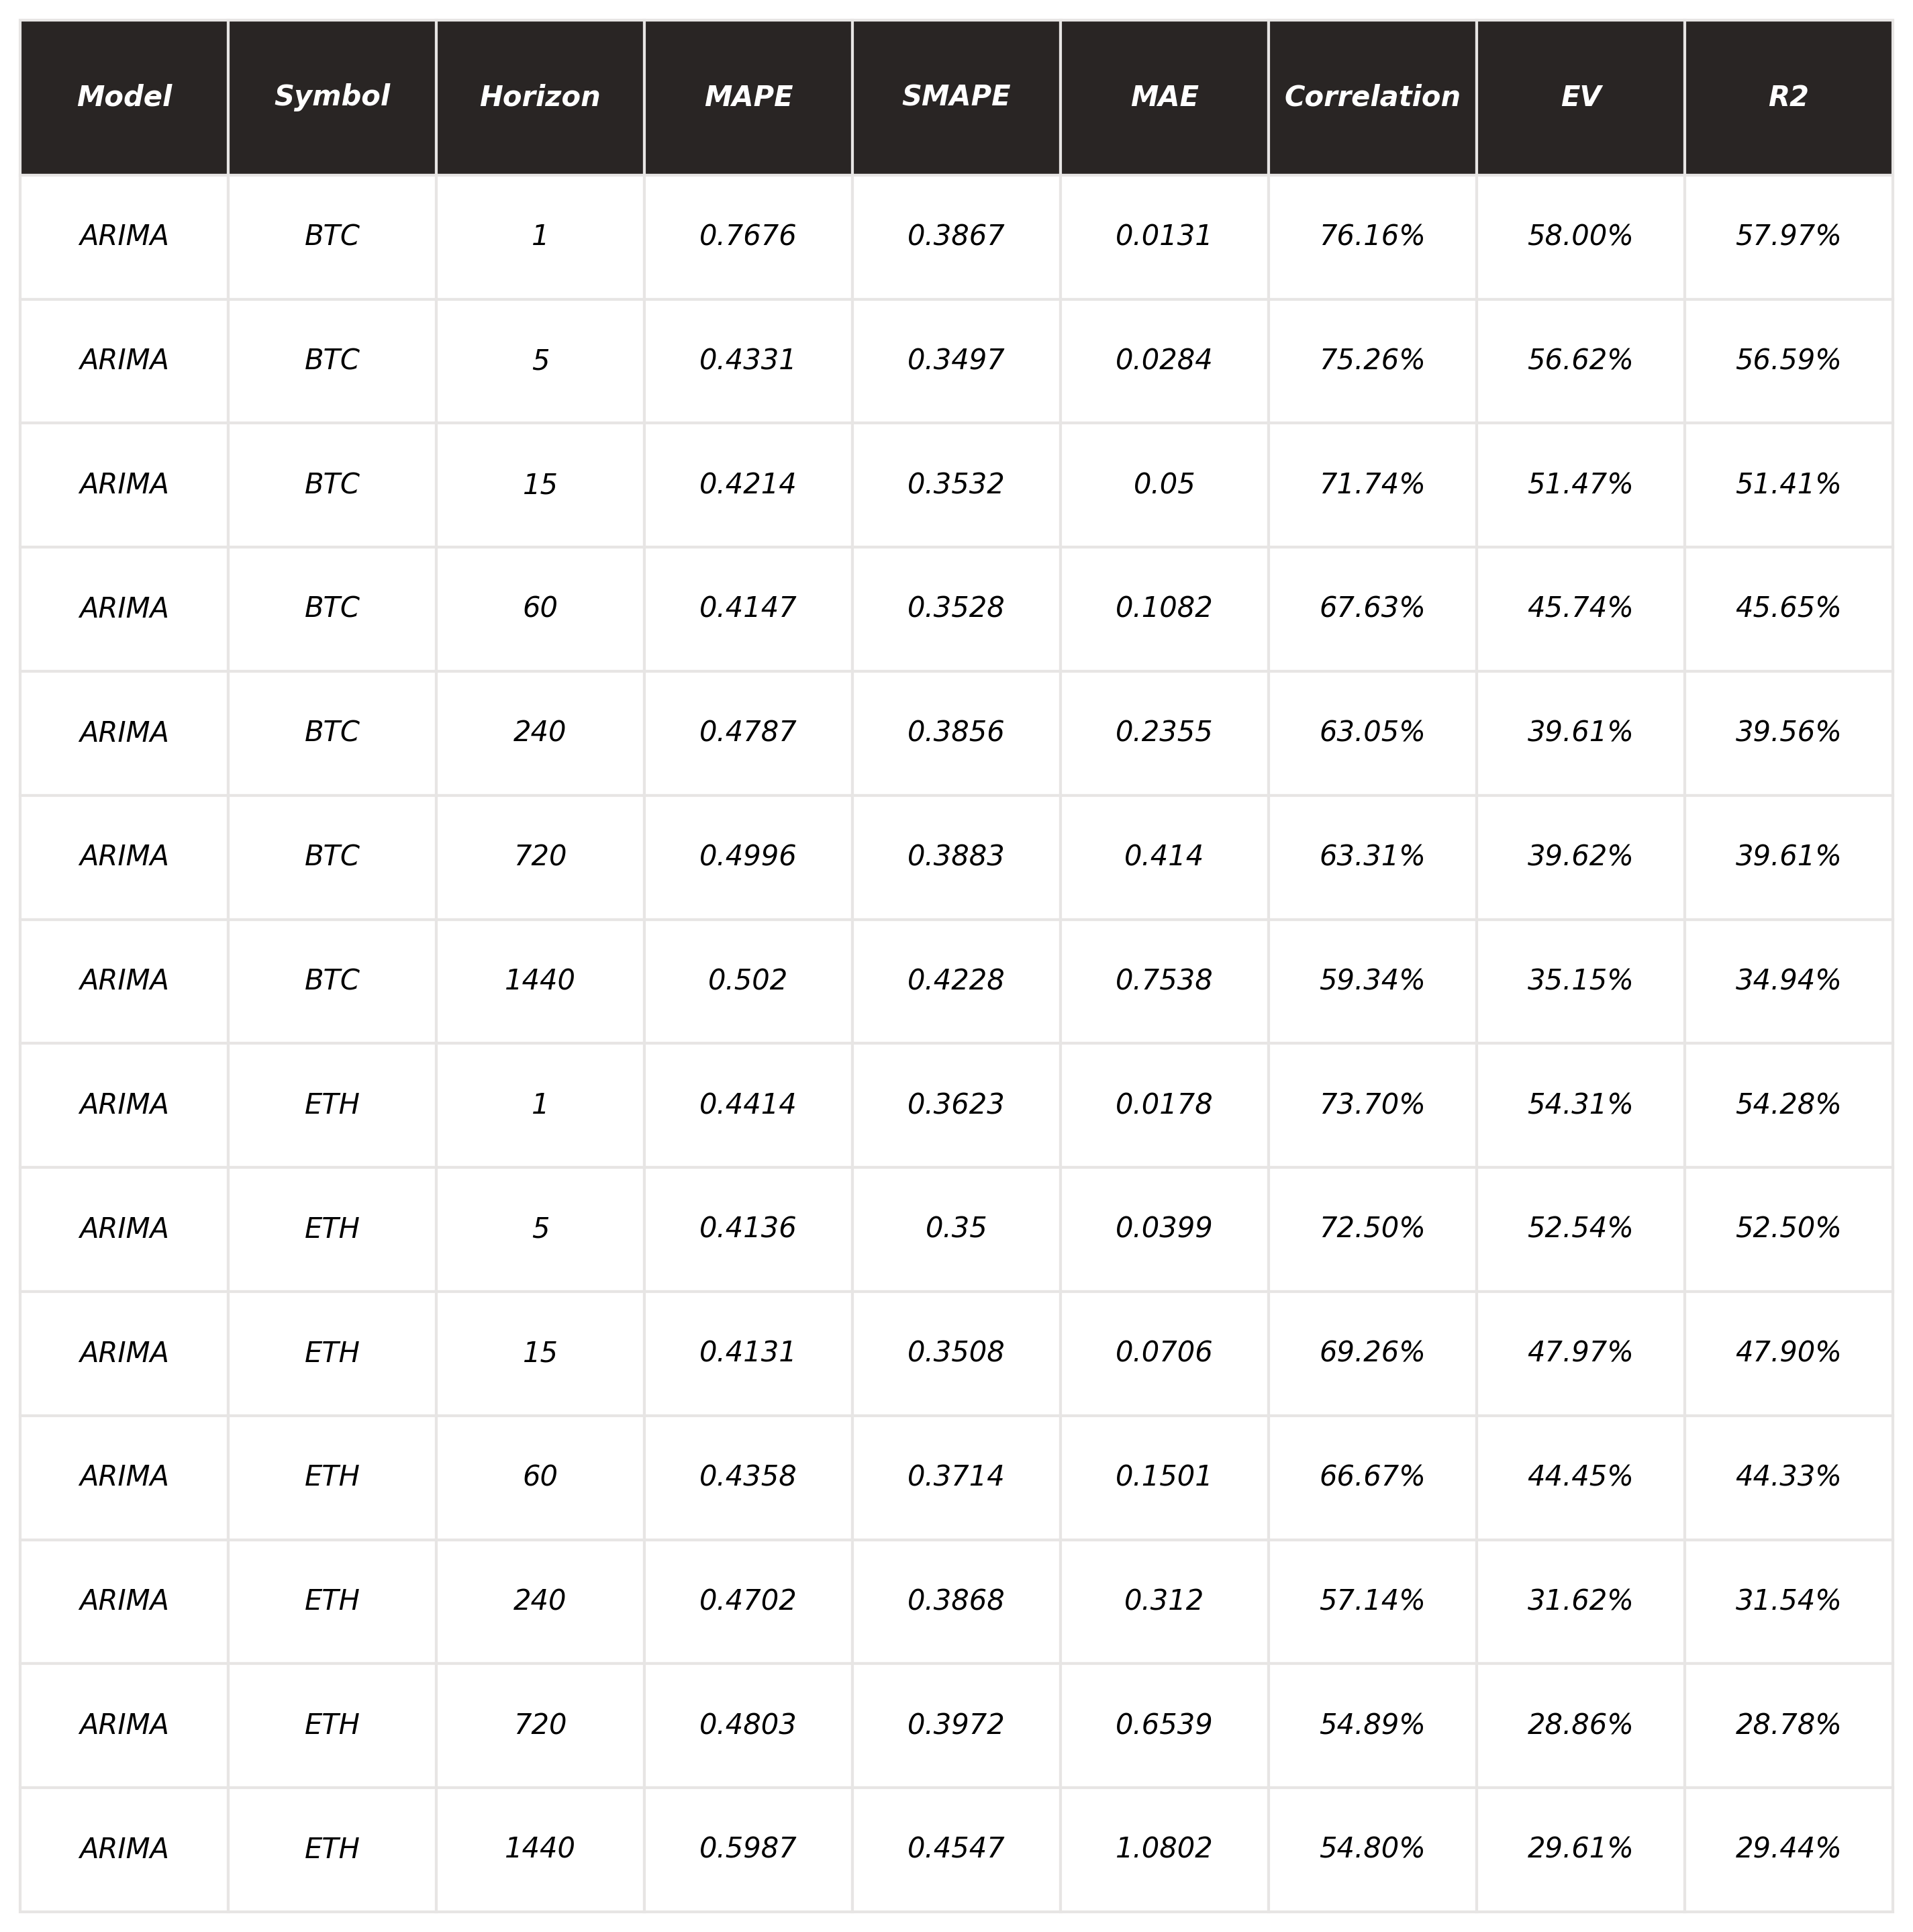
\includegraphics[width=.99\columnwidth]{img/_KPI_ARIMA.png}
		\captionof{figure}{ARIMA KPIs}
		\label{fig:_KPI_ARIMA}
		\justifying
		\medskip
		
		The results show that ARIMA performs reasonably well at short horizons, with performance degrading as the forecast horizon lengthens:
		\begin{itemize}
			\item At the 1-minute horizon, ETH forecasts achieve a MAPE of 0.4414 and SMAPE of 0.3623, with a strong correlation of 73.7\% and \( R^2 = 54.28\% \).
			\item At 5 and 15 minutes, metrics remain competitive (\( R^2 = 52.50\% \) and \( 47.90\% \), respectively), though predictive power tapers.
			\item For longer horizons (60–1440 minutes), performance declines steadily. At 1440 minutes (24 hours), \( R^2 \) drops to 29.44\%, with a significant increase in MAE (1.0802) and lower correlation (54.80\%).
		\end{itemize}
		
		Overall, ARIMA demonstrates greater effectiveness at capturing short-term volatility patterns in ETH, but struggles with long-range dependencies and non-linear behaviors, especially as volatility aggregates over time.
		
		\subsection{HAR Models}
		
		To evaluate volatility forecasting using the Heterogeneous Autoregressive (HAR) model, we leveraged historical ETH and BTC minute-level price data. Volatility was computed as the standard deviation of log returns across multiple horizons: 1, 5, 15, 60, 240, 720, and 1440 minutes.
		
		\smallskip
		
		The HAR framework captures volatility persistence across different temporal scales by incorporating lagged volatilities from multiple horizons. Specifically, for each forecast horizon \( h \), the model uses lagged values from all horizons equal to or longer than \( h \), such as \( \text{std}_{5}, \text{std}_{15}, \text{std}_{60}, \ldots \), forming a feature set that reflects market memory at varying resolutions.
		
		Model training and evaluation were performed using a monthly rolling-window approach, spanning October 1, 2024, to April 1, 2025. For each forecast month, the model was retrained using all prior data to emulate a live forecasting environment. Predictions were generated iteratively and aggregated across all months.
		
		\centering
		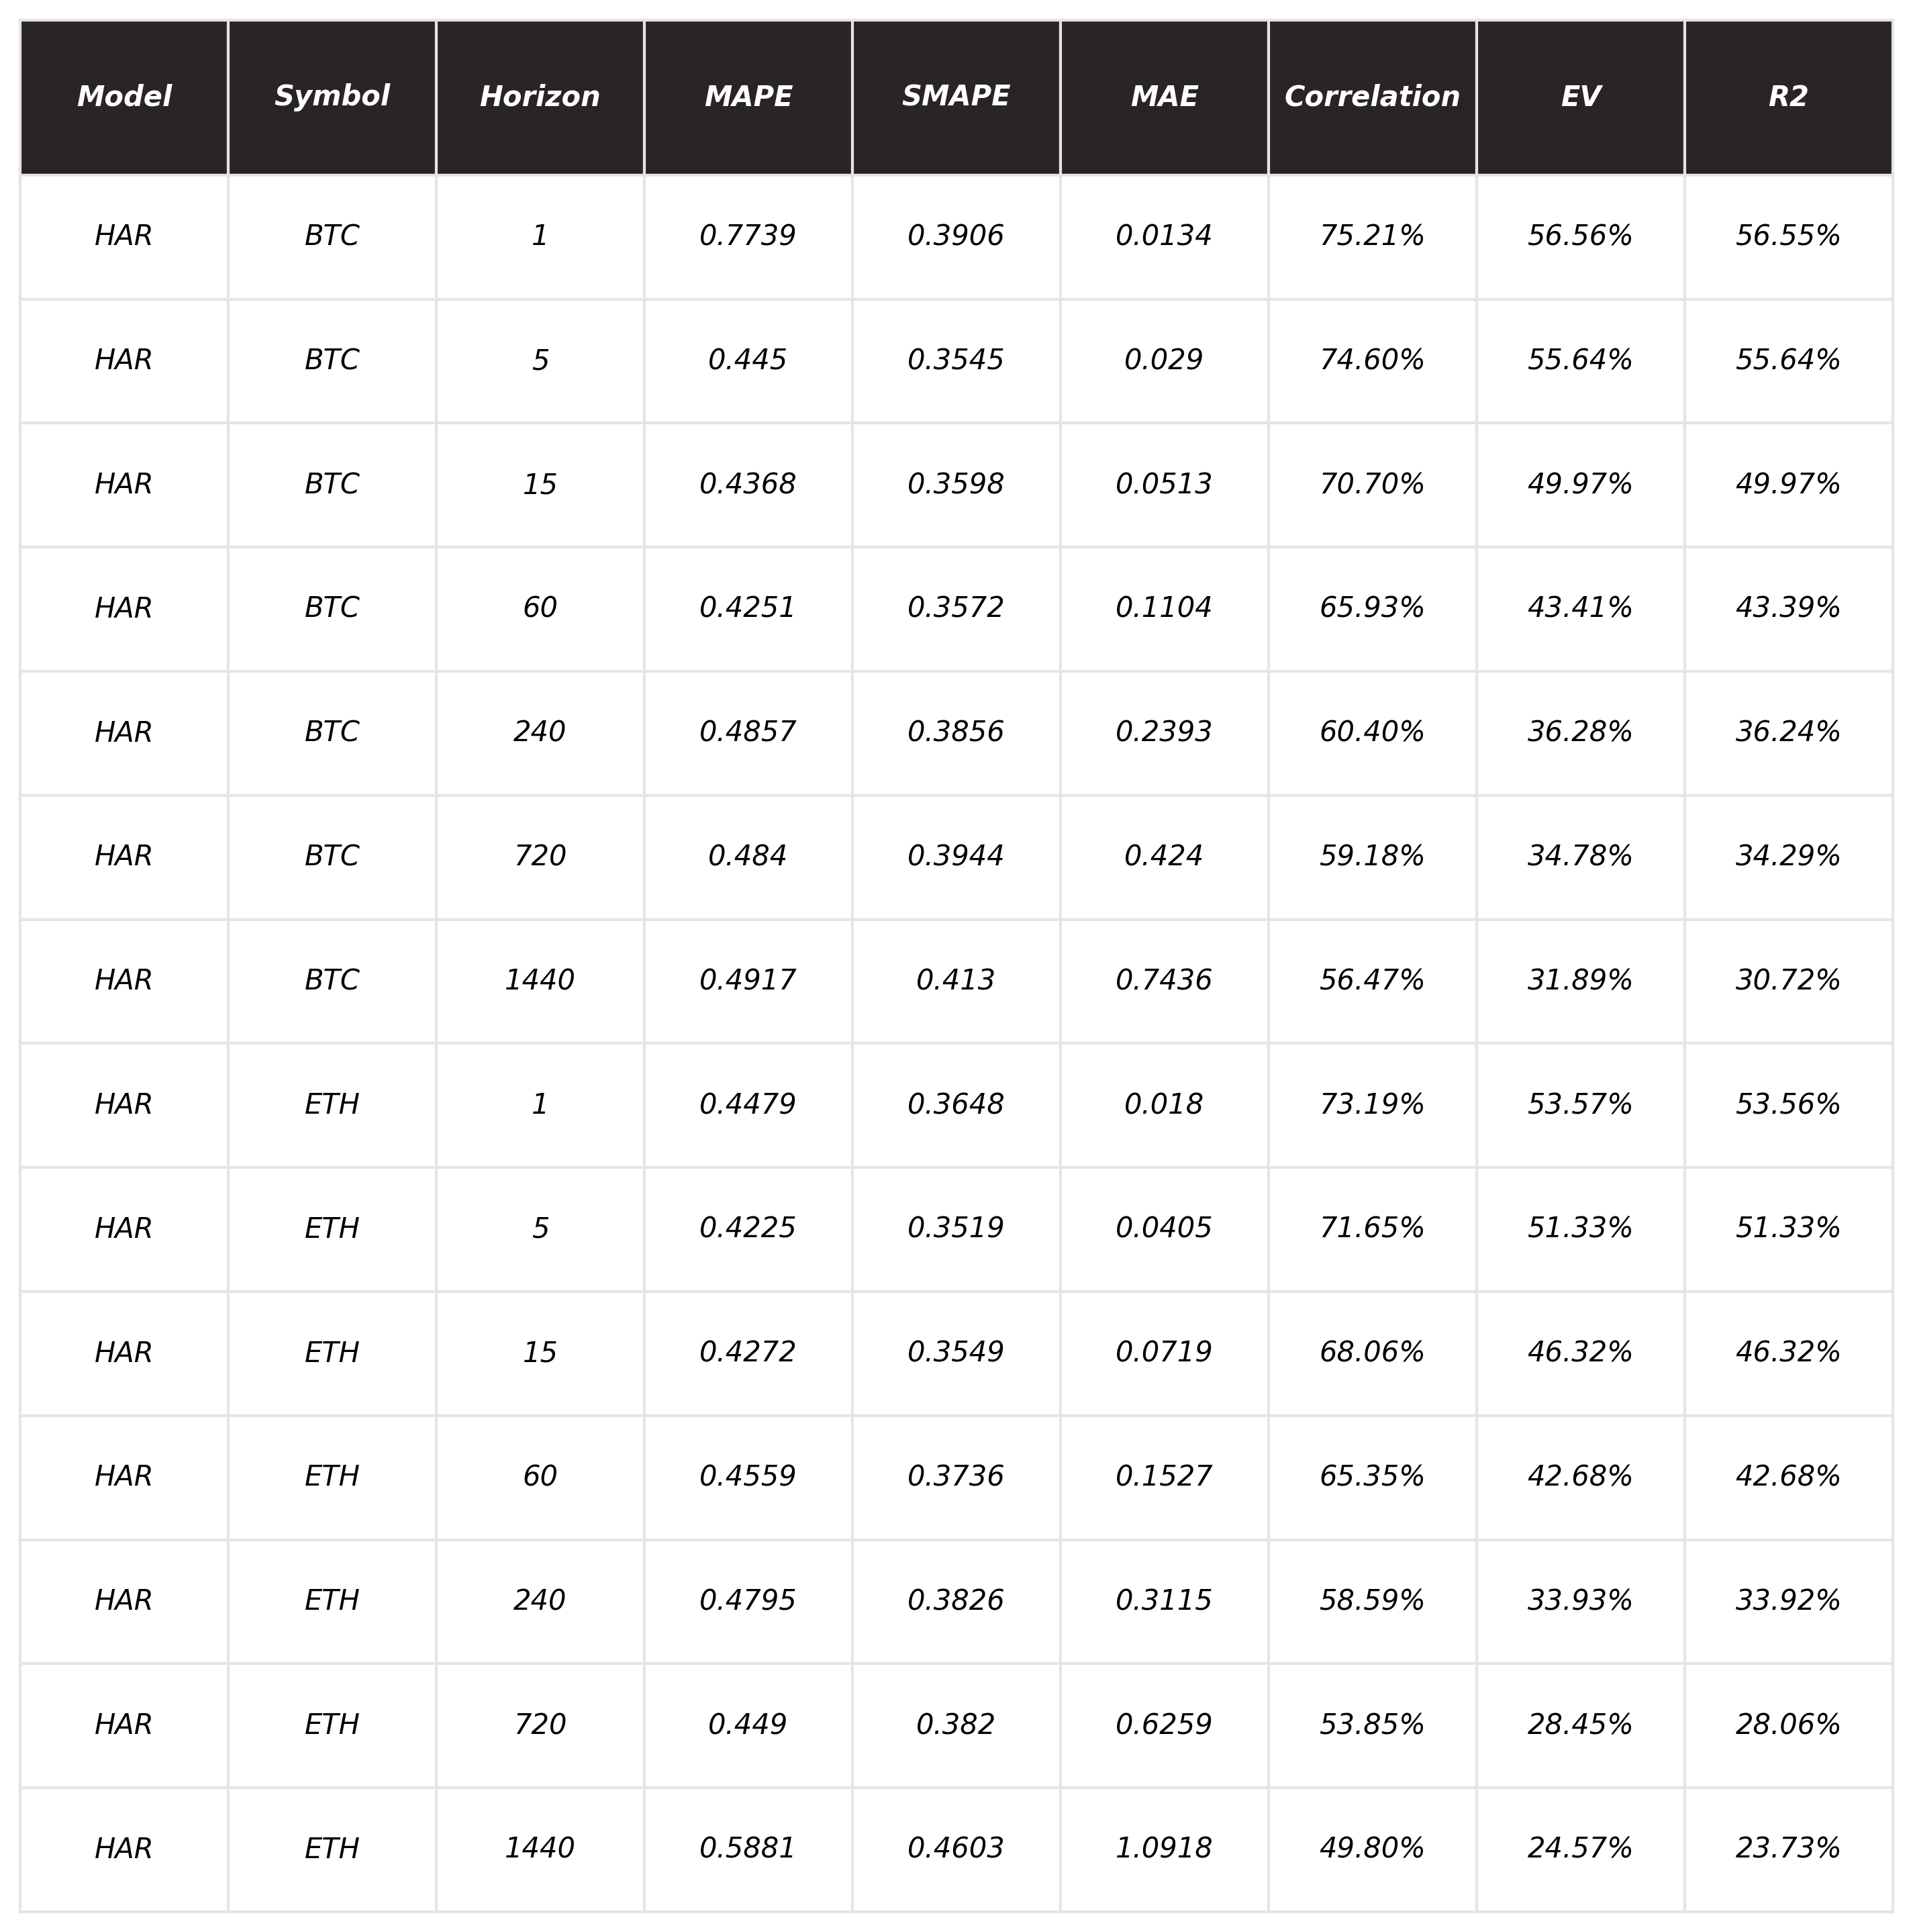
\includegraphics[width=.99\columnwidth]{img/_KPI_HAR.png}
		\captionof{figure}{HAR KPIs}
		\label{fig:_KPI_HAR}
		\justifying
		\medskip
		
		\textbf{Ethereum (ETH)} results demonstrate that the HAR model offers competitive accuracy at short-to-medium horizons, though performance weakens at longer timeframes:
		\begin{itemize}
			\item At the 1-minute horizon, ETH forecasts yield a MAPE of 0.4479 and SMAPE of 0.3648, with a correlation of 73.19\% and \( R^2 = 53.56\% \).
			\item At 5 and 15 minutes, performance remains relatively strong with \( R^2 = 51.33\% \) and \( 46.32\% \), respectively, indicating HAR's ability to leverage multi-scale temporal patterns.
			\item For extended horizons (60–1440 minutes), model effectiveness declines. At the 1440-minute (24-hour) horizon, \( R^2 \) drops to 23.73\%, accompanied by higher MAE (1.0918) and reduced correlation (49.80\%).
		\end{itemize}
		
		These findings suggest that while HAR effectively captures volatility persistence at finer granularities, its linear structure may limit its ability to model long-range or non-linear effects, highlighting the potential benefits of more adaptive models discussed later in this study.
		
		\subsection{ARCH Models}
		
		ARCH-type models form a core class of econometric techniques for modeling and forecasting time-varying volatility. These models are designed to capture the conditional heteroskedasticity observed in financial returns, where periods of high and low volatility tend to cluster over time. In this study, we assess six prominent variants: ARCH, GARCH, EGARCH, FIGARCH, APARCH, and GJR-GARCH. Each was applied to log returns of Ethereum (ETH) computed at horizons of 60, 240, 720, and 1440 minutes.
		
		\medskip
		
		For each model, rolling forecasts were generated monthly between October 1, 2024, and April 1, 2025. The models were refitted using only prior data to simulate a realistic out-of-sample prediction setting. Forecasts were compared against realized volatility (standard deviation) using key performance metrics including MAPE, SMAPE, MAE, correlation, and \( R^2 \).
		
		\subsubsection{ARCH}
		\centering
		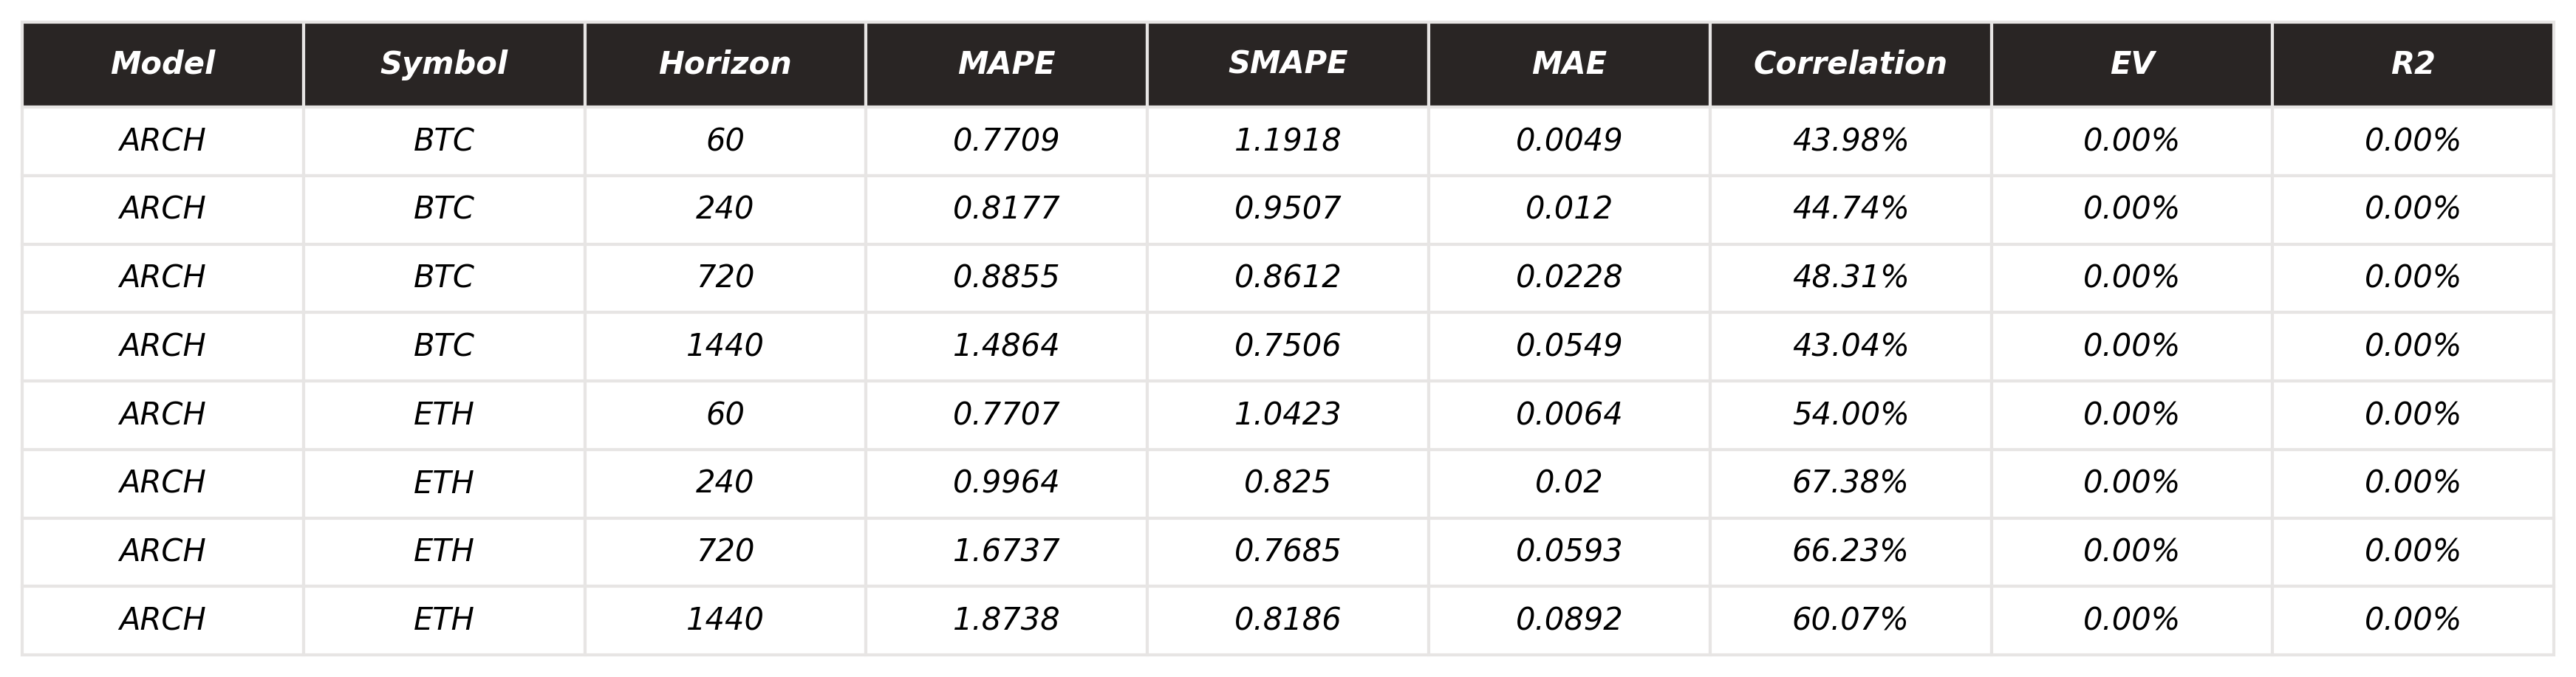
\includegraphics[width=.95\columnwidth]{img/_KPI_ARCH.png}
		\captionof{figure}{ARCH KPIs}
		\label{fig:_KPI_ARCH}
		\justifying
		\medskip
		
		The basic ARCH(1) model captures time-varying volatility through lagged squared returns. While conceptually foundational, its lack of moving average terms limits its ability to smooth volatility estimates.
		
		\begin{itemize}
			\item At 60 minutes, ARCH achieves a moderate MAPE of 0.7707 and correlation of 54.00\%.
			\item At longer horizons (e.g., 1440 minutes), accuracy degrades, with \( \text{MAPE} = 1.8738 \) and low predictive power (\( R^2 = 0 \)).
		\end{itemize}
		
		\subsubsection{GARCH}
		\centering
		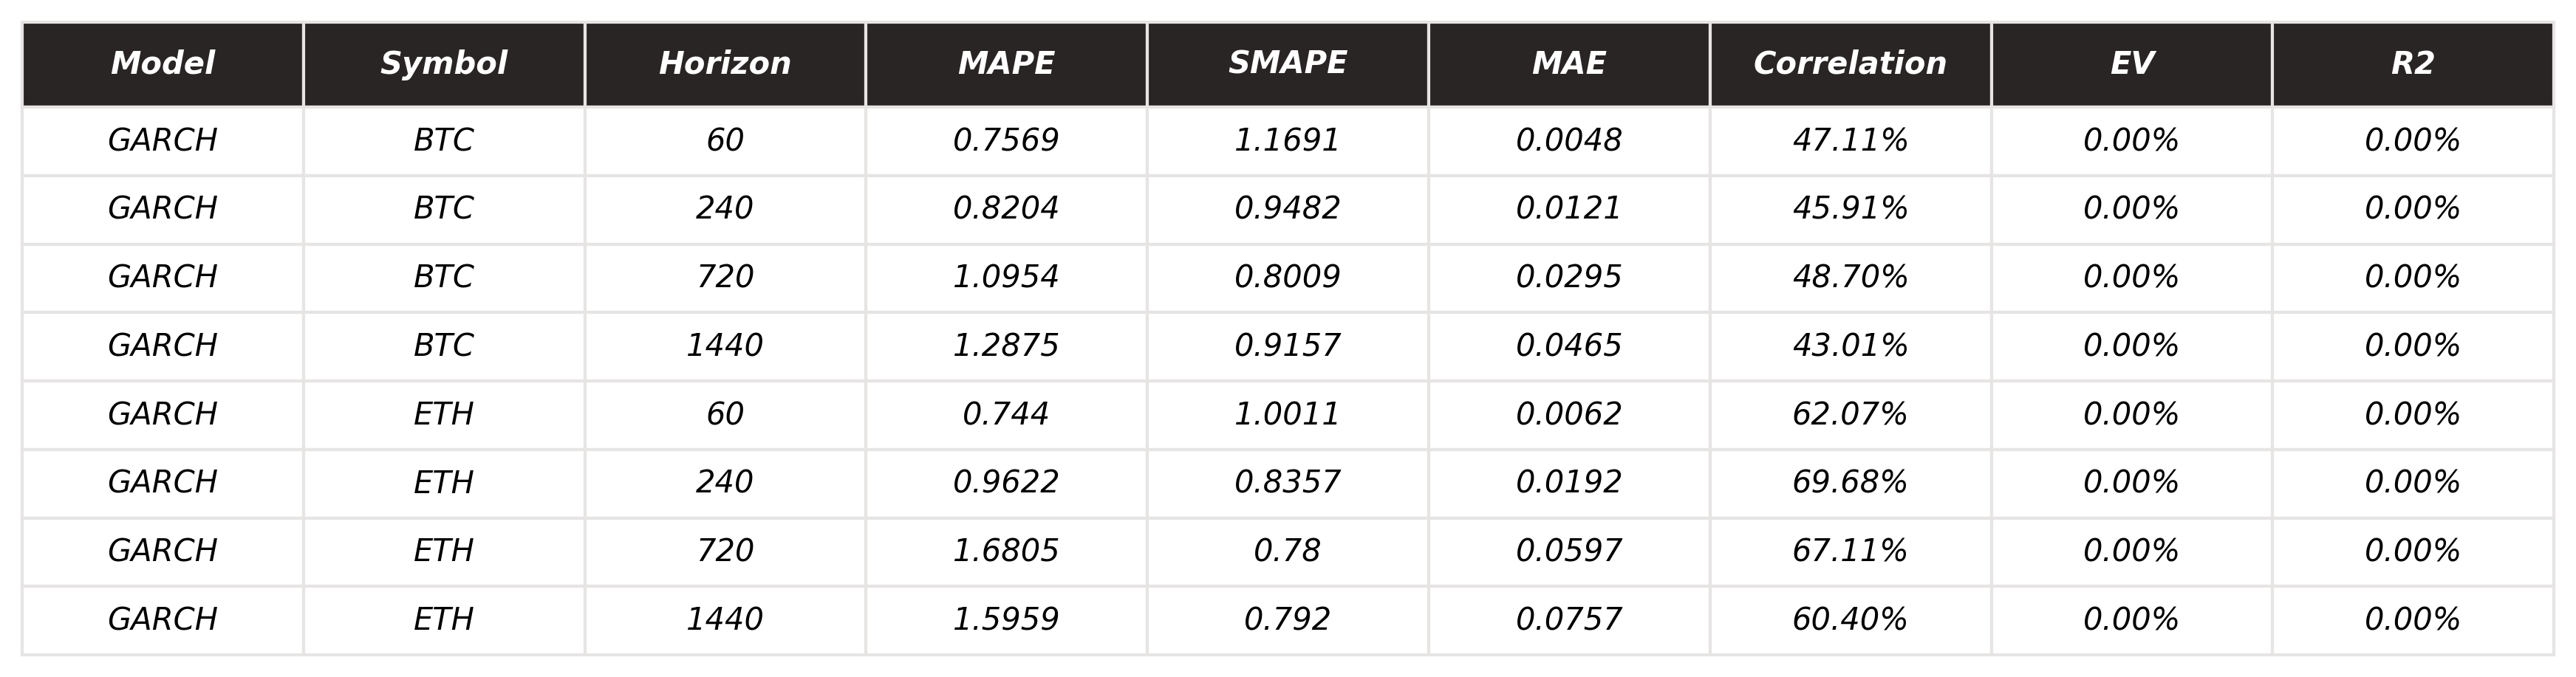
\includegraphics[width=.95\columnwidth]{img/_KPI_GARCH.png}
		\captionof{figure}{GARCH KPIs}
		\label{fig:_KPI_GARCH}
		\justifying
		\medskip
		
		GARCH(1,1) improves upon ARCH by including lagged conditional variance terms, providing smoother and more persistent volatility estimates.
		
		\begin{itemize}
			\item Performance improves slightly over ARCH, with 60-minute forecasts showing lower MAPE (0.7440) and stronger correlation (62.07\%).
			\item However, at 1440 minutes, \( R^2 \) remains effectively zero, suggesting limited value for long-range crypto forecasting.
		\end{itemize}
		
		\subsubsection{EGARCH}
		\centering
		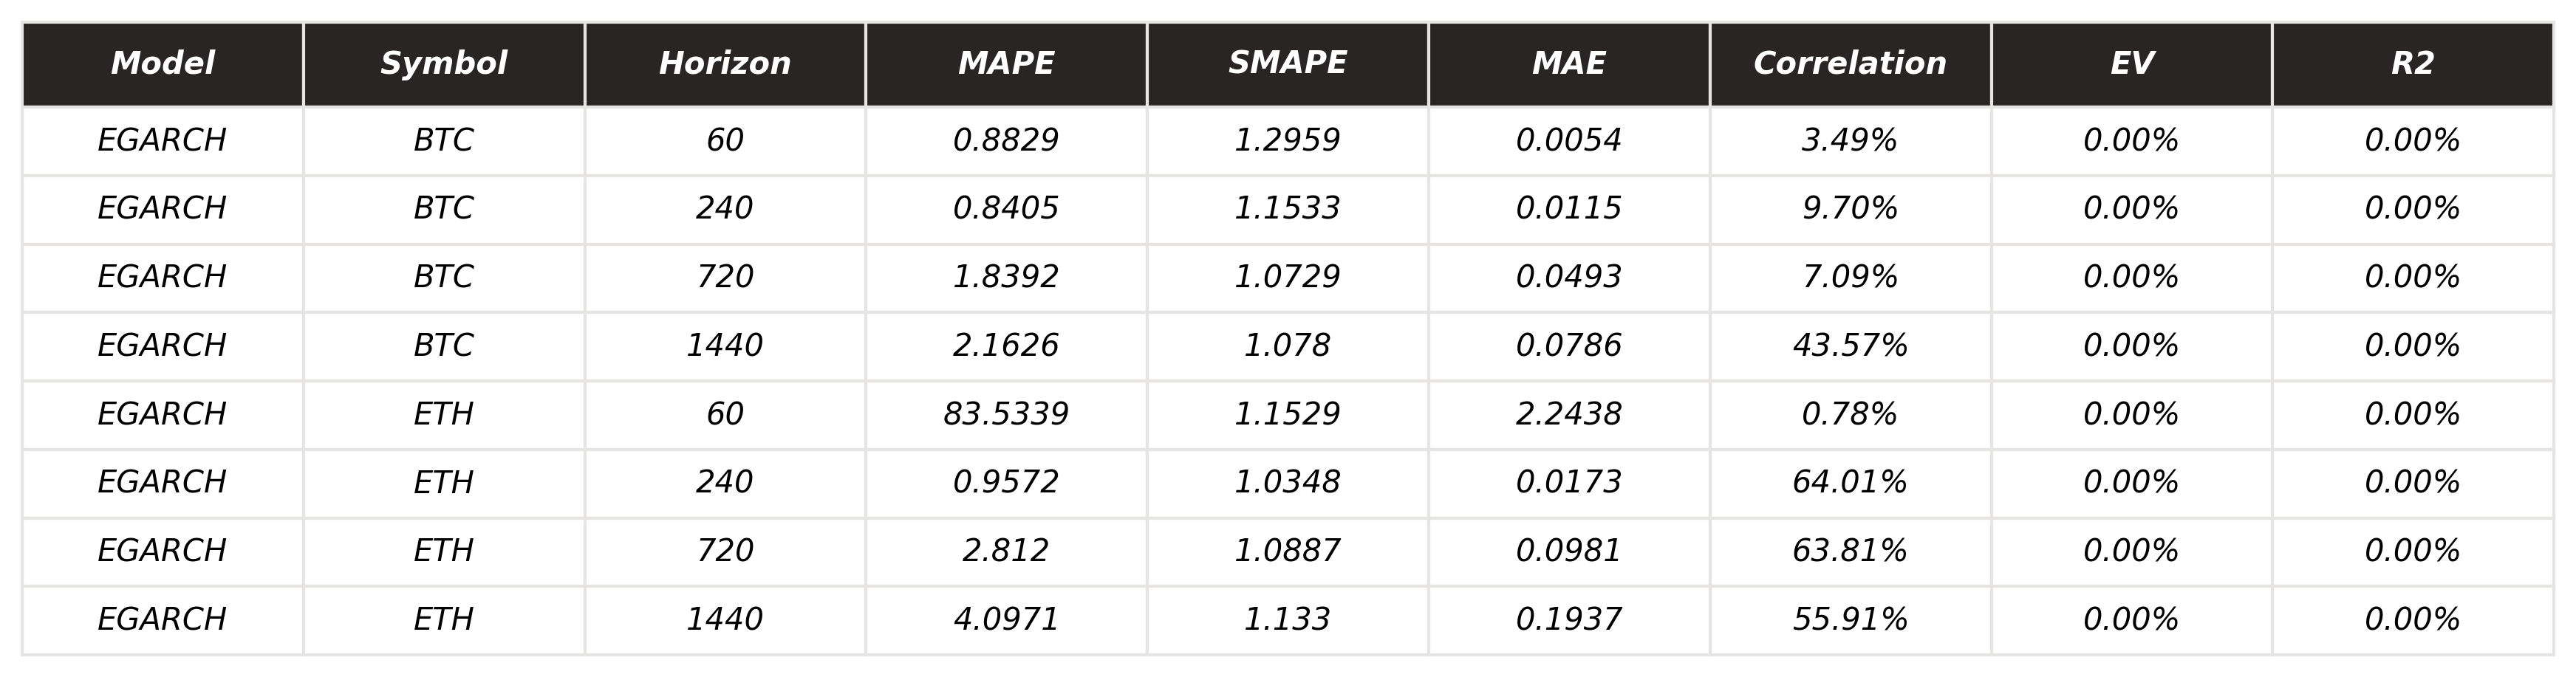
\includegraphics[width=.95\columnwidth]{img/_KPI_EGARCH.png}
		\captionof{figure}{EGARCH KPIs}
		\label{fig:_KPI_EGARCH}
		\justifying
		\medskip
		
		EGARCH introduces asymmetry, allowing the model to distinguish between positive and negative shocks. It captures leverage effects often observed in equity markets.
		
		\begin{itemize}
			\item At 60 minutes, results are unstable, with a massive MAPE of 83.5339 and extremely low correlation (0.78\%), suggesting numerical instability or misspecification.
			\item Performance slightly stabilizes at longer horizons, though remains weak overall.
		\end{itemize}
		
		\subsubsection{FIGARCH}
		\centering
		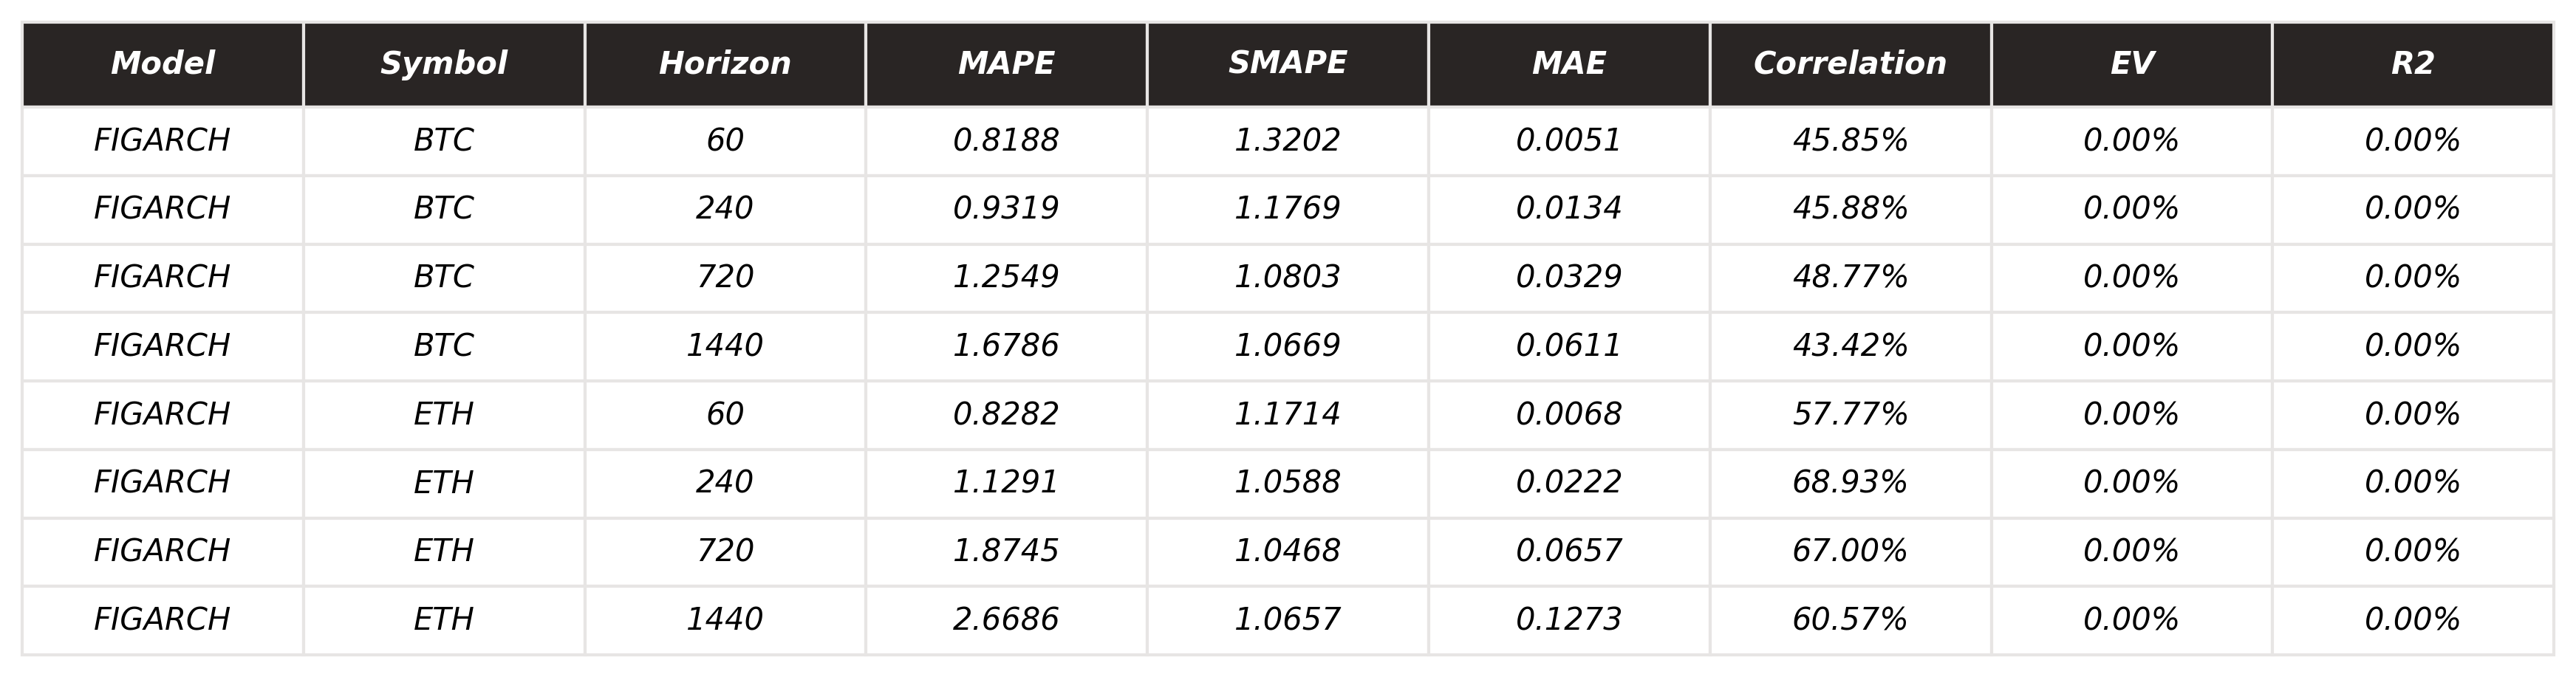
\includegraphics[width=.95\columnwidth]{img/_KPI_FIGARCH.png}
		\captionof{figure}{FIGARCH KPIs}
		\label{fig:_KPI_FIGARCH}
		\justifying
		\medskip
		
		FIGARCH models incorporate long memory by allowing fractional differencing of volatility. This structure is theoretically suitable for assets with persistent volatility.
		
		\begin{itemize}
			\item Shows consistent moderate performance across horizons, e.g., 60-minute MAPE = 0.8282, correlation = 57.77\%.
			\item At 1440 minutes, FIGARCH achieves better correlation (60.57\%) than most peers, indicating relative robustness in long-horizon settings.
		\end{itemize}
		
		\subsubsection{APARCH}
		\centering
		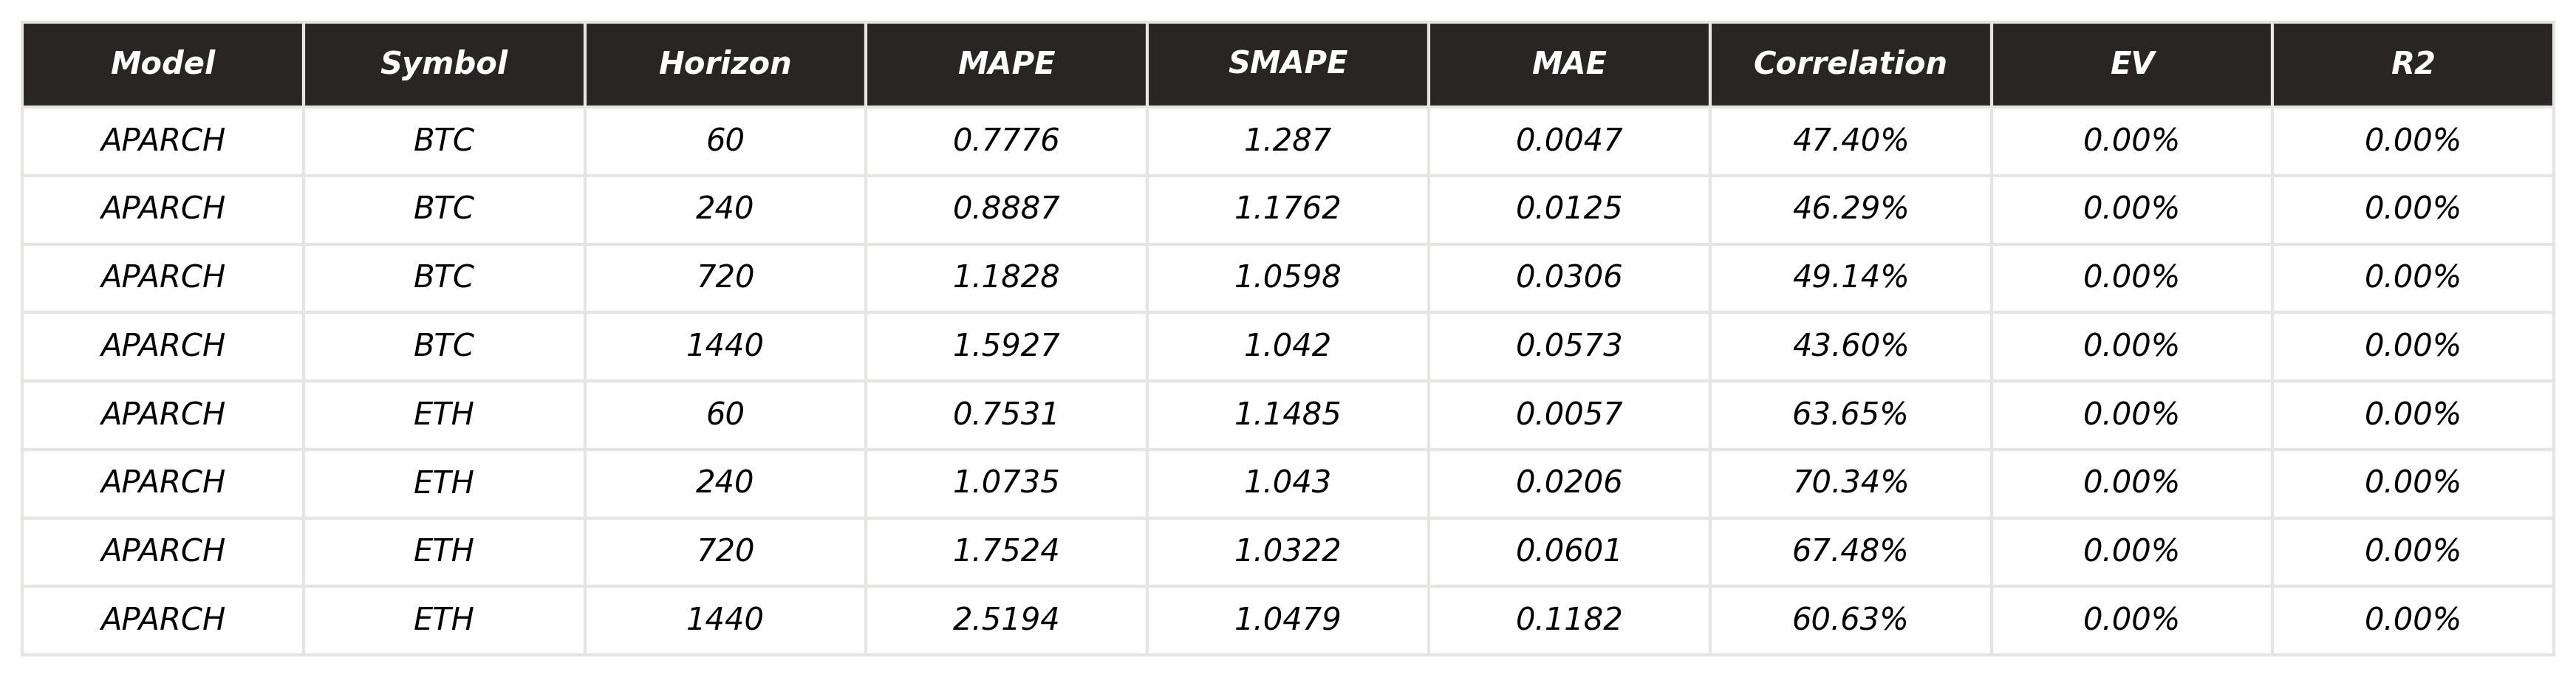
\includegraphics[width=.95\columnwidth]{img/_KPI_APARCH.png}
		\captionof{figure}{APARCH KPIs}
		\label{fig:_KPI_APARCH}
		\justifying
		\medskip
		
		The APARCH model generalizes GARCH by adding asymmetry and a flexible power parameter. It’s tailored for capturing fat-tailed and skewed return distributions.
		
		\begin{itemize}
			\item At 60 minutes, APARCH outperforms basic models with a correlation of 63.65\% and MAPE of 0.7531.
			\item However, performance deteriorates rapidly at higher horizons, with a 1440-minute MAPE of 2.5194 and no measurable \( R^2 \).
		\end{itemize}
		
		\subsubsection{GJR-GARCH}
		\centering
		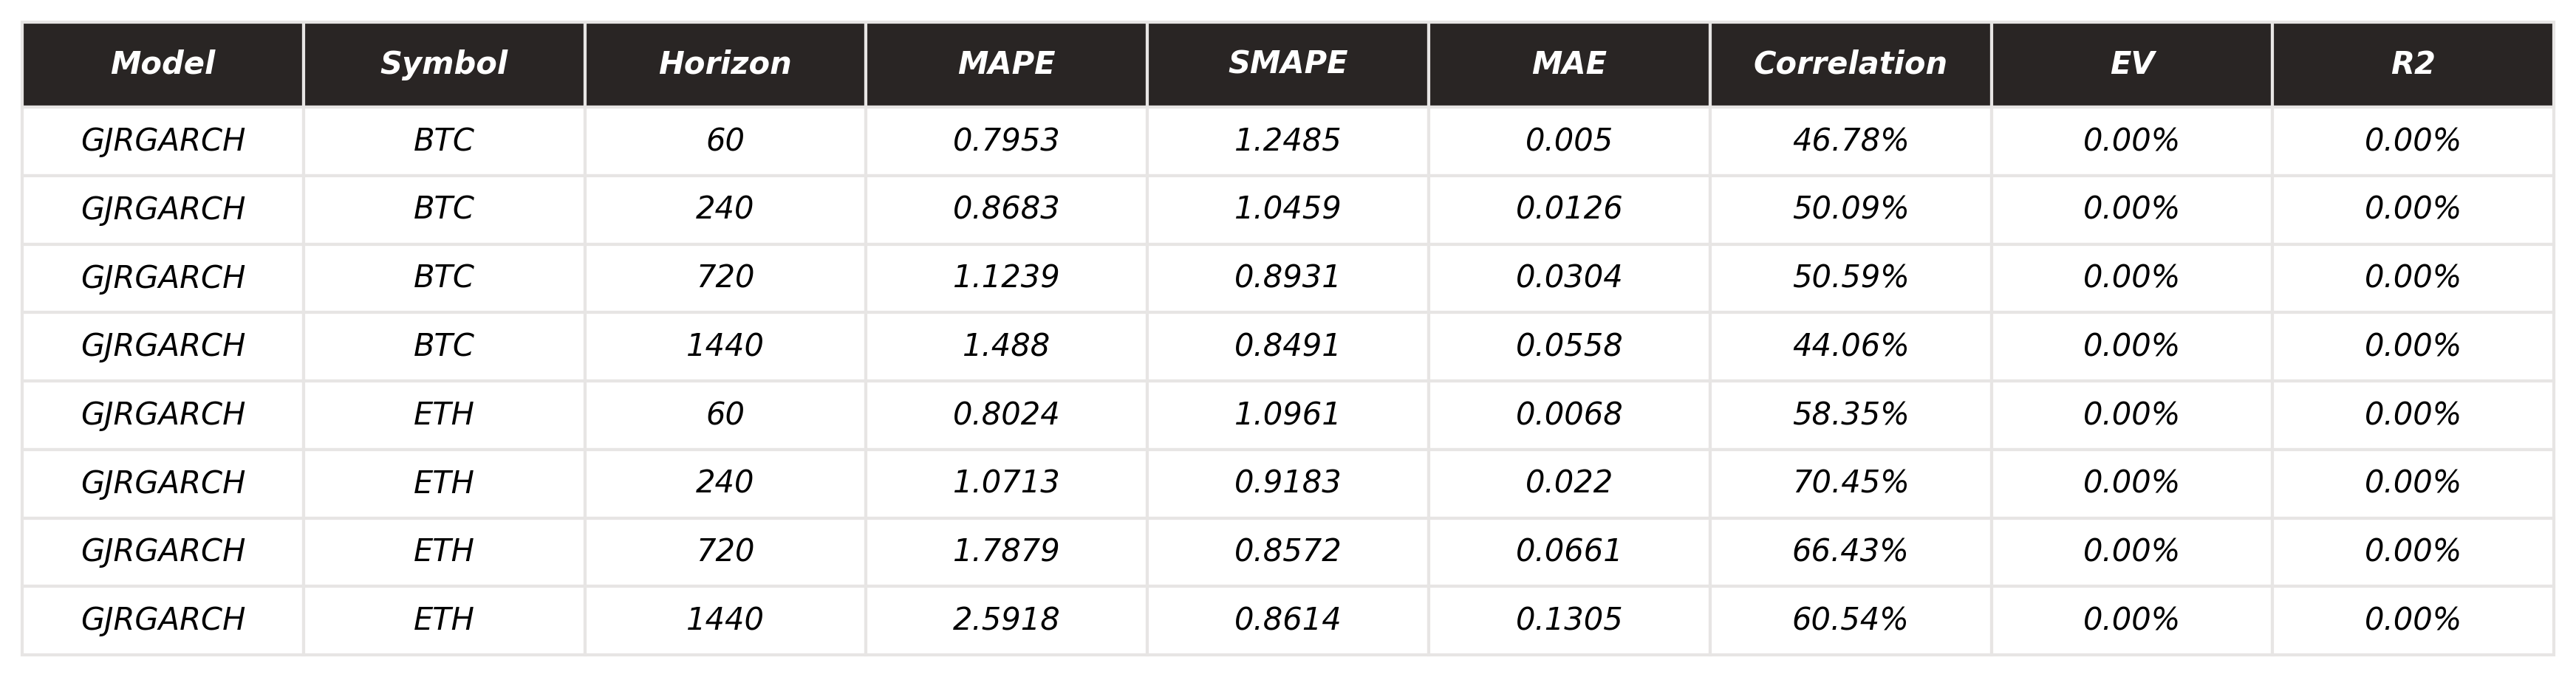
\includegraphics[width=.95\columnwidth]{img/_KPI_GJRGARCH.png}
		\captionof{figure}{GJR-GARCH KPIs}
		\label{fig:_KPI_GJRGARCH}
		\justifying
		\medskip
		
		GJR-GARCH adds asymmetry via a leverage term (like EGARCH), offering improved modeling of volatility spikes following negative returns.
		
		\begin{itemize}
			\item Offers comparable accuracy to APARCH: at 240 minutes, correlation reaches 70.45\%.
			\item At 1440 minutes, maintains consistent performance with correlation of 60.54\%, among the highest of the group.
		\end{itemize}
		
		\textbf{Summary:} While all ARCH-type models capture short-term volatility dynamics to varying degrees, none exhibit meaningful explanatory power at daily horizons (\( R^2 \approx 0 \)). FIGARCH and GJR-GARCH demonstrate slightly better long-horizon robustness. The inability of these models to explain long-range Ethereum volatility highlights the need for more flexible, non-linear architectures—such as hybrid models or deep learning approaches—explored in the following sections.
		
	\end{multicols}

\newpage
\bibliography{references}

\newpage

\section{Appendix}

\subsection{Ethereum Visualization}

\medskip
\centering
\includegraphics[width=.90\columnwidth]{img/_ETH ARIMA.png}
\captionof{figure}{Etherum ARIMA Forecasts Visualisation}
\label{fig:_ETH_ARIMA}

\medskip
\centering
\includegraphics[width=.90\columnwidth]{img/_ETH HAR.png}
\captionof{figure}{Etherum HAR Forecasts Visualisation}
\label{fig:_ETH_HAR}

\medskip
\centering
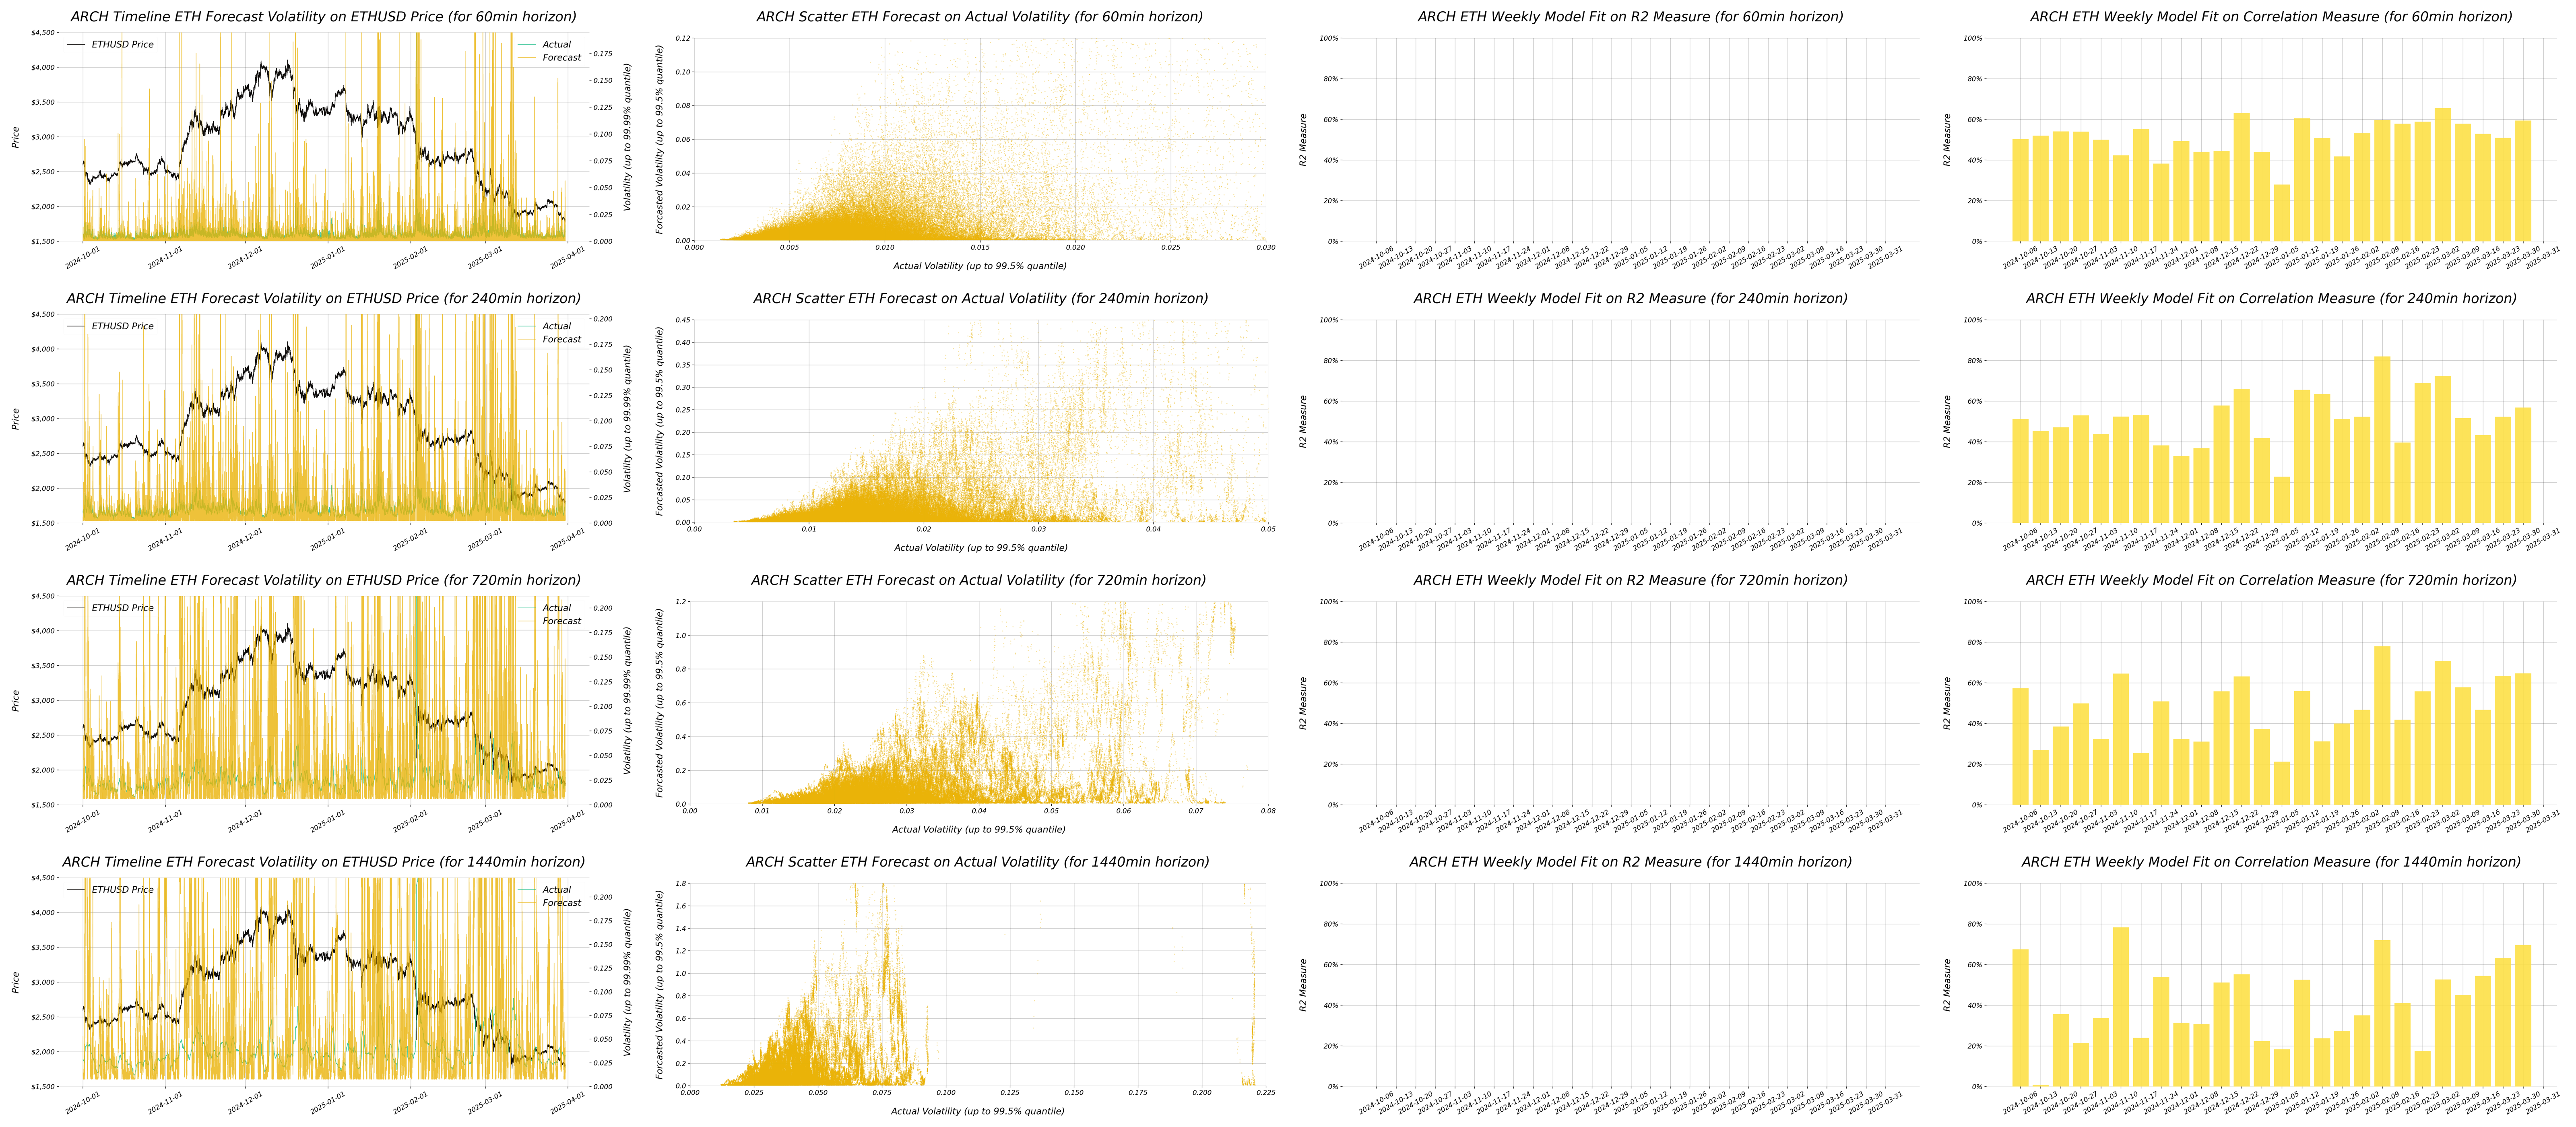
\includegraphics[width=.90\columnwidth]{img/_ETH ARCH.png}
\captionof{figure}{Etherum ARCH Forecasts Visualisation}
\label{fig:_ETH_ARCH}

\medskip
\centering
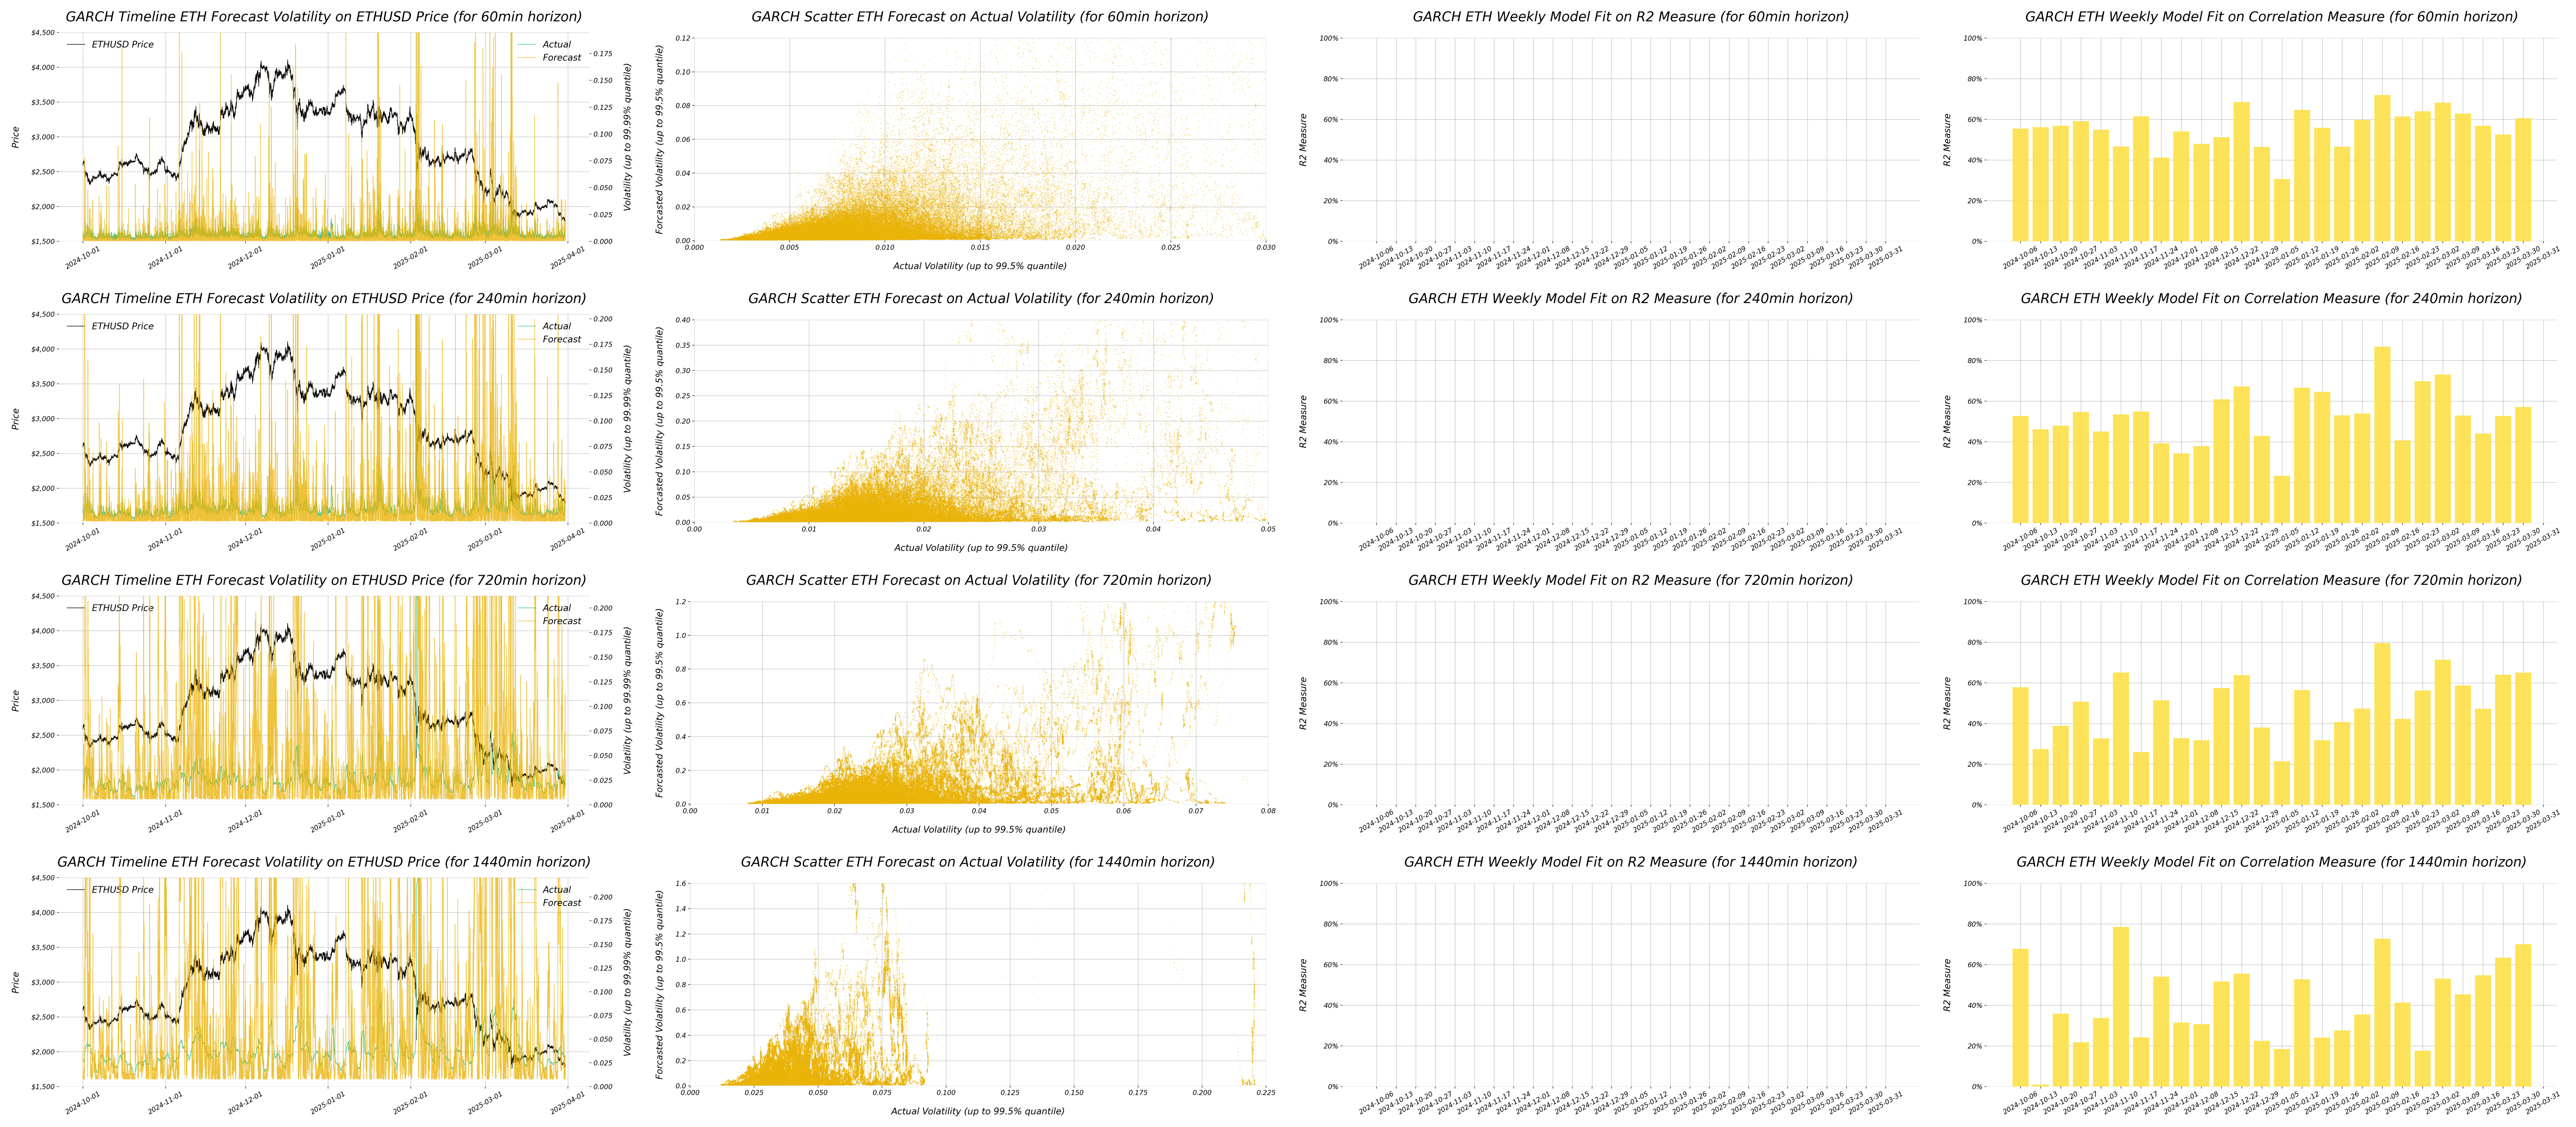
\includegraphics[width=.90\columnwidth]{img/_ETH GARCH.png}
\captionof{figure}{Ethereum GARCH Forecasts Visualisation}
\label{fig:_ETH_GARCH}

\medskip
\centering
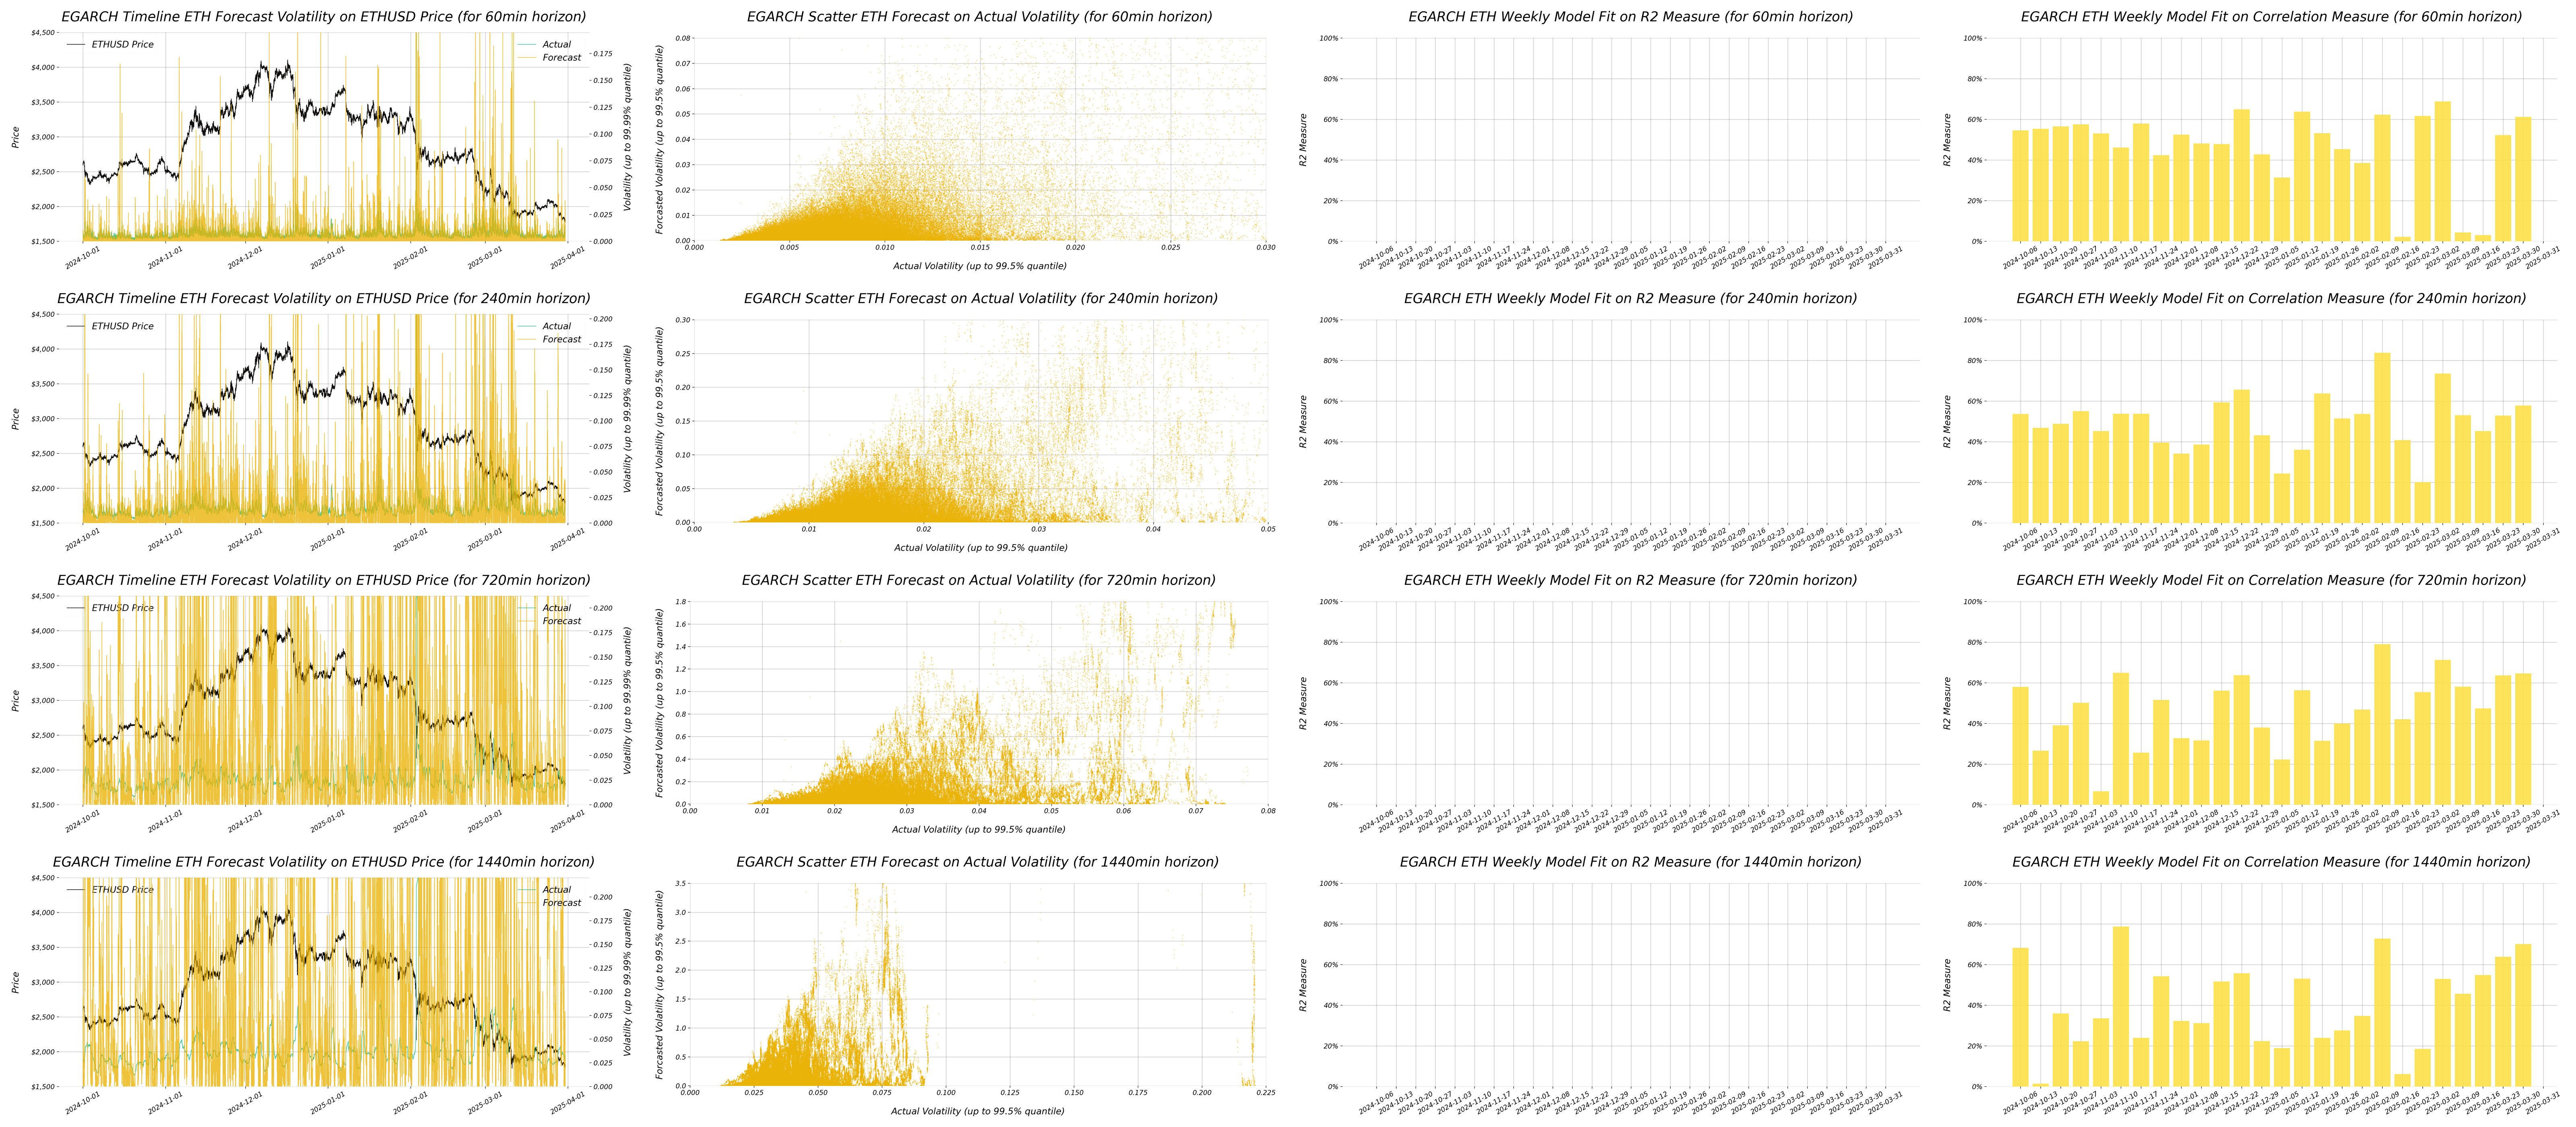
\includegraphics[width=.90\columnwidth]{img/_ETH EGARCH.png}
\captionof{figure}{Ethereum EGARCH Forecasts Visualisation}
\label{fig:_ETH_EGARCH}

\medskip
\centering
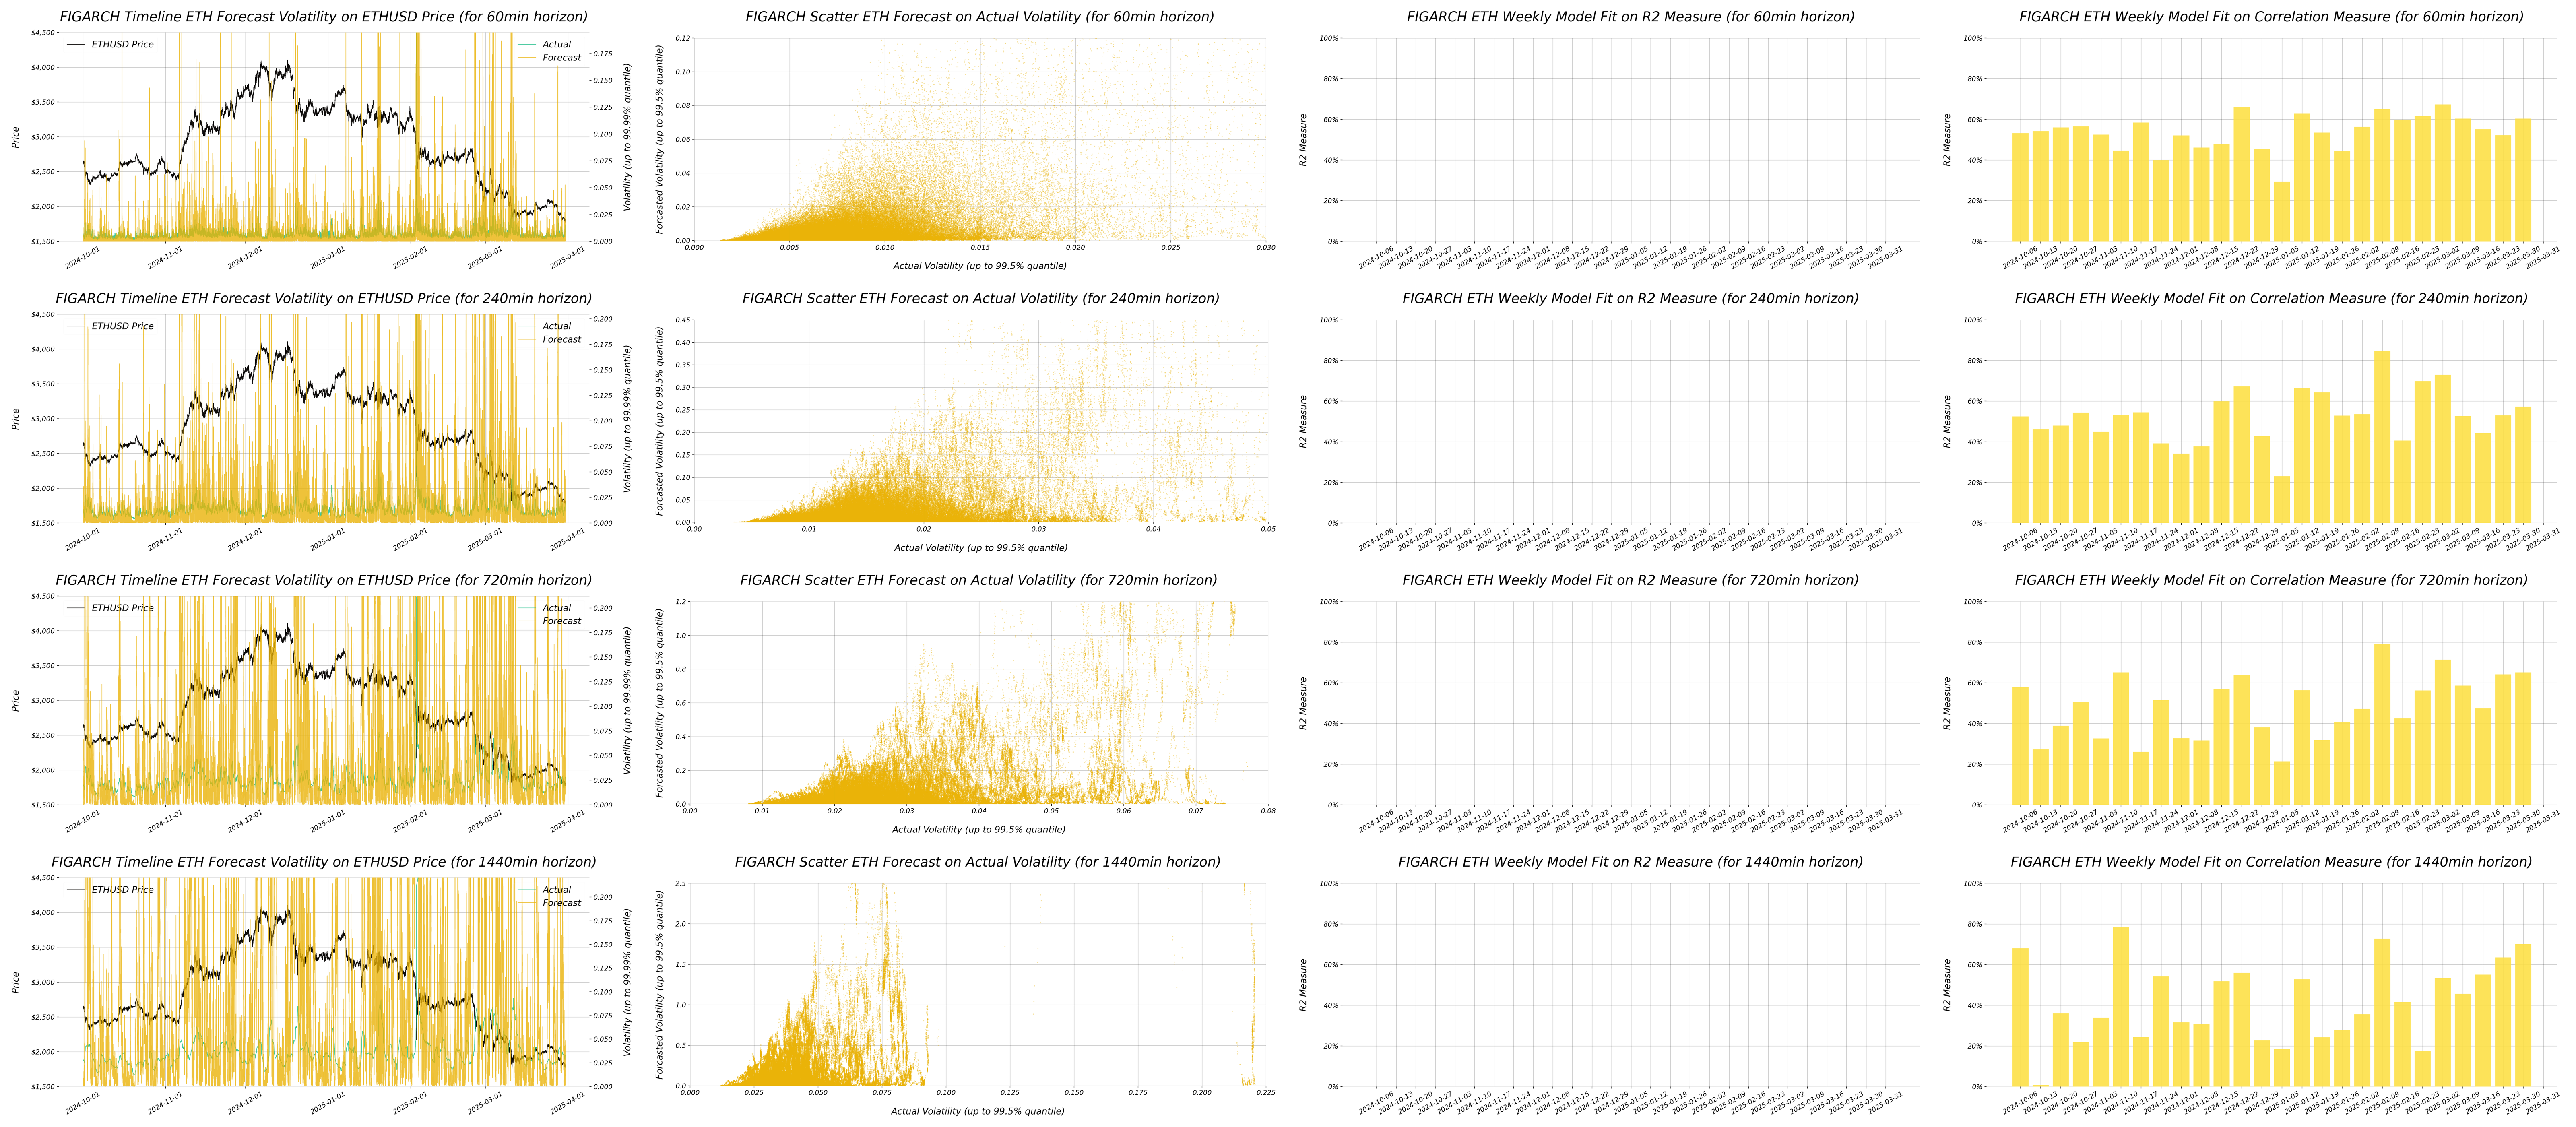
\includegraphics[width=.90\columnwidth]{img/_ETH FIGARCH.png}
\captionof{figure}{Ethereum FIGARCH Forecasts Visualisation}
\label{fig:_ETH_FIGARCH}

\medskip
\centering
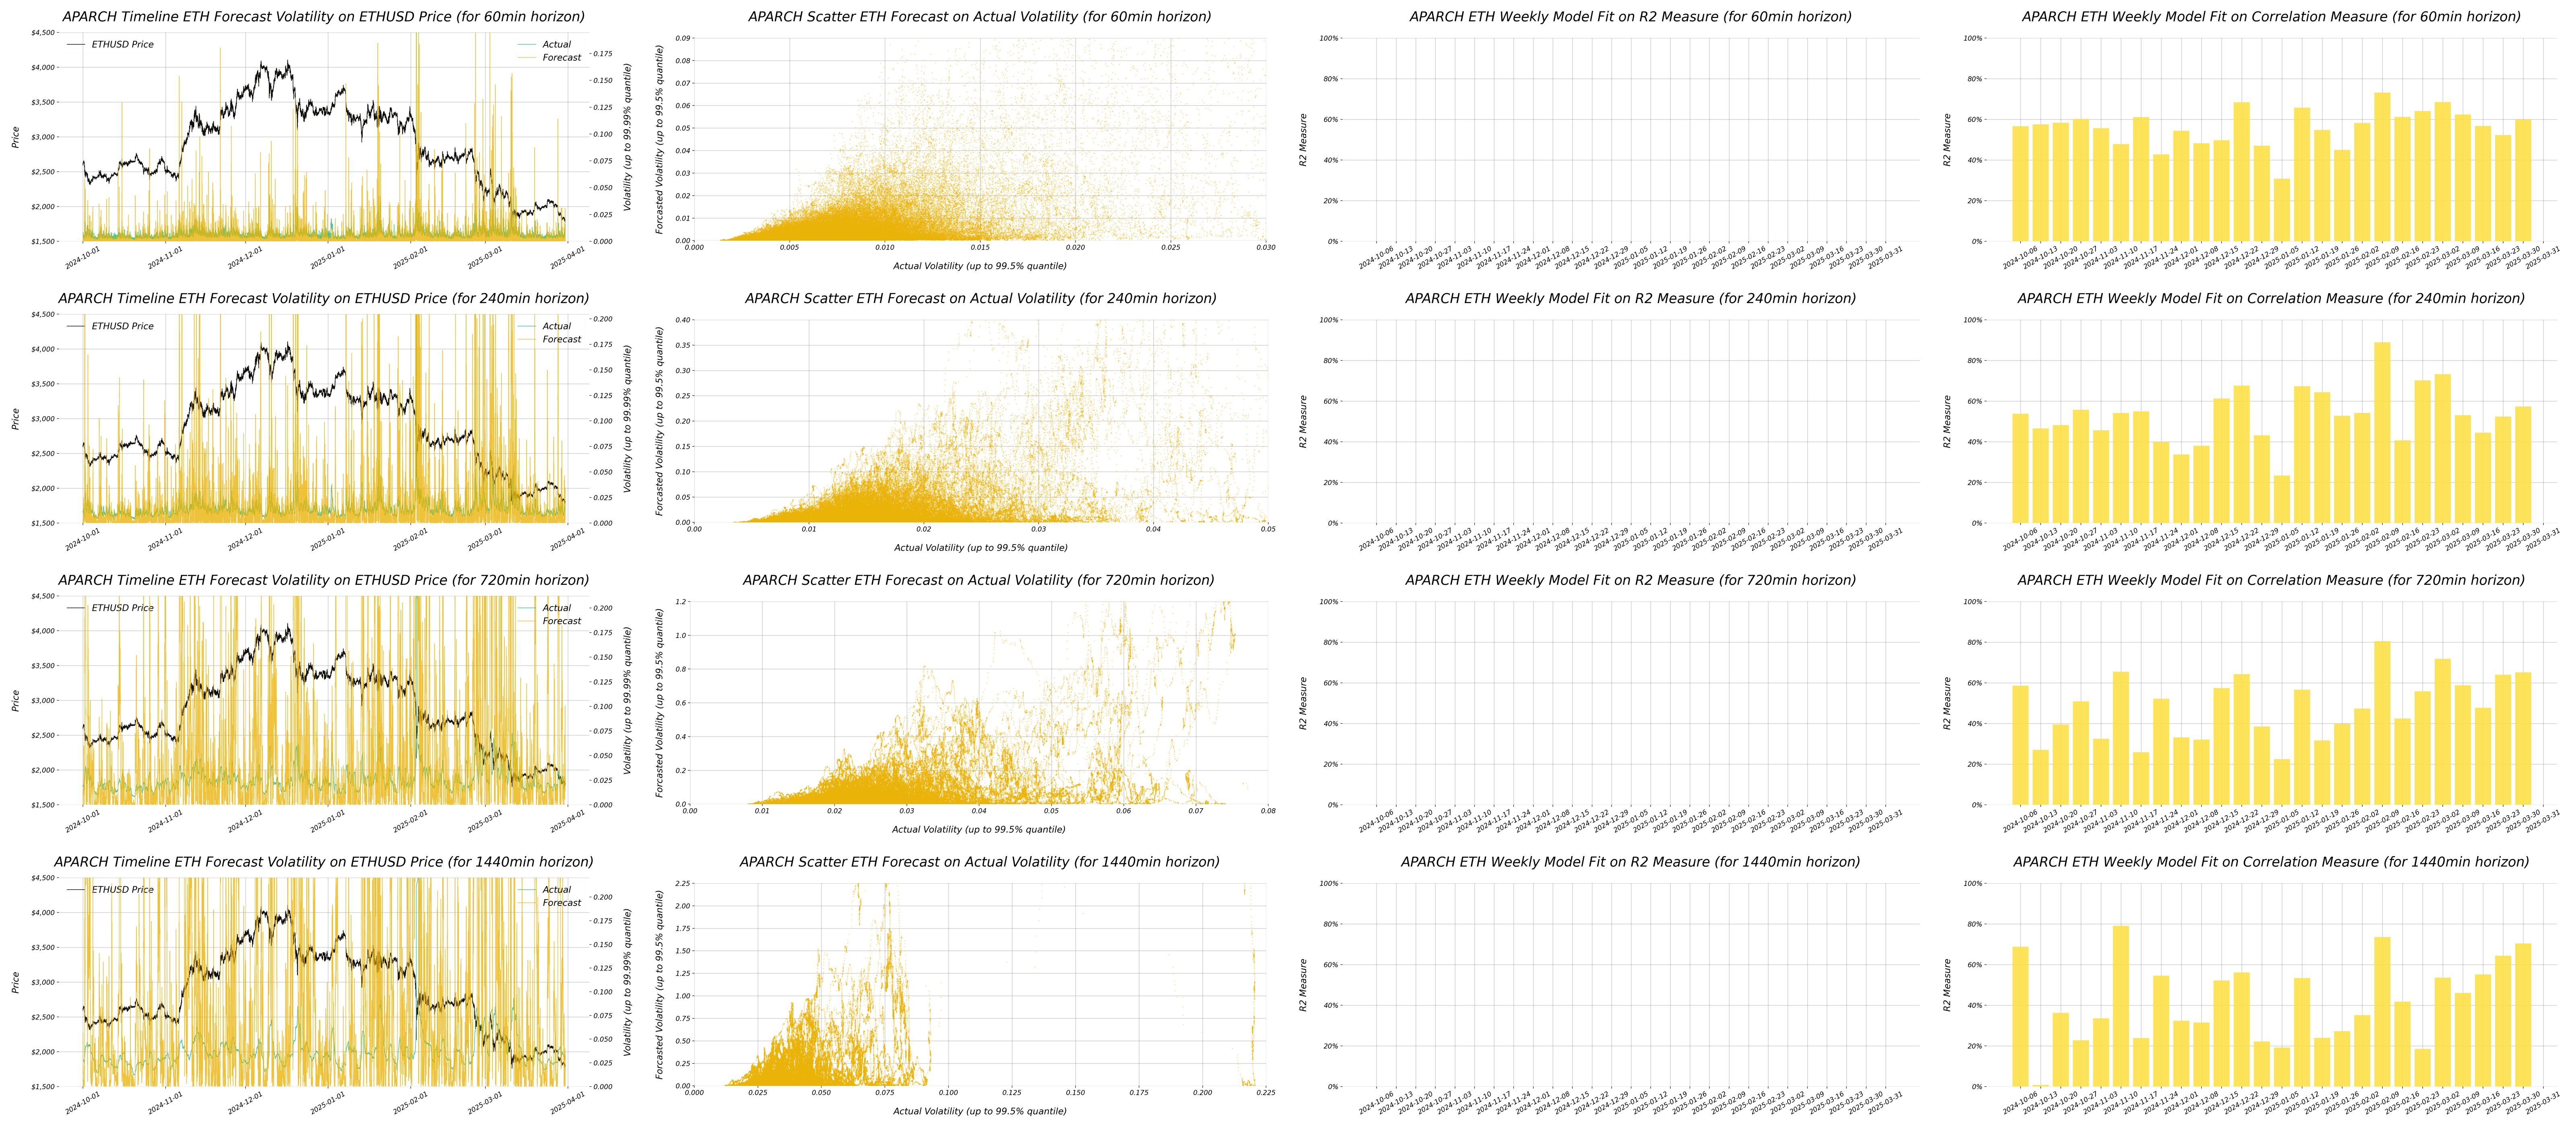
\includegraphics[width=.90\columnwidth]{img/_ETH APARCH.png}
\captionof{figure}{Ethereum APARCH Forecasts Visualisation}
\label{fig:_ETH_APARCH}

\medskip
\centering
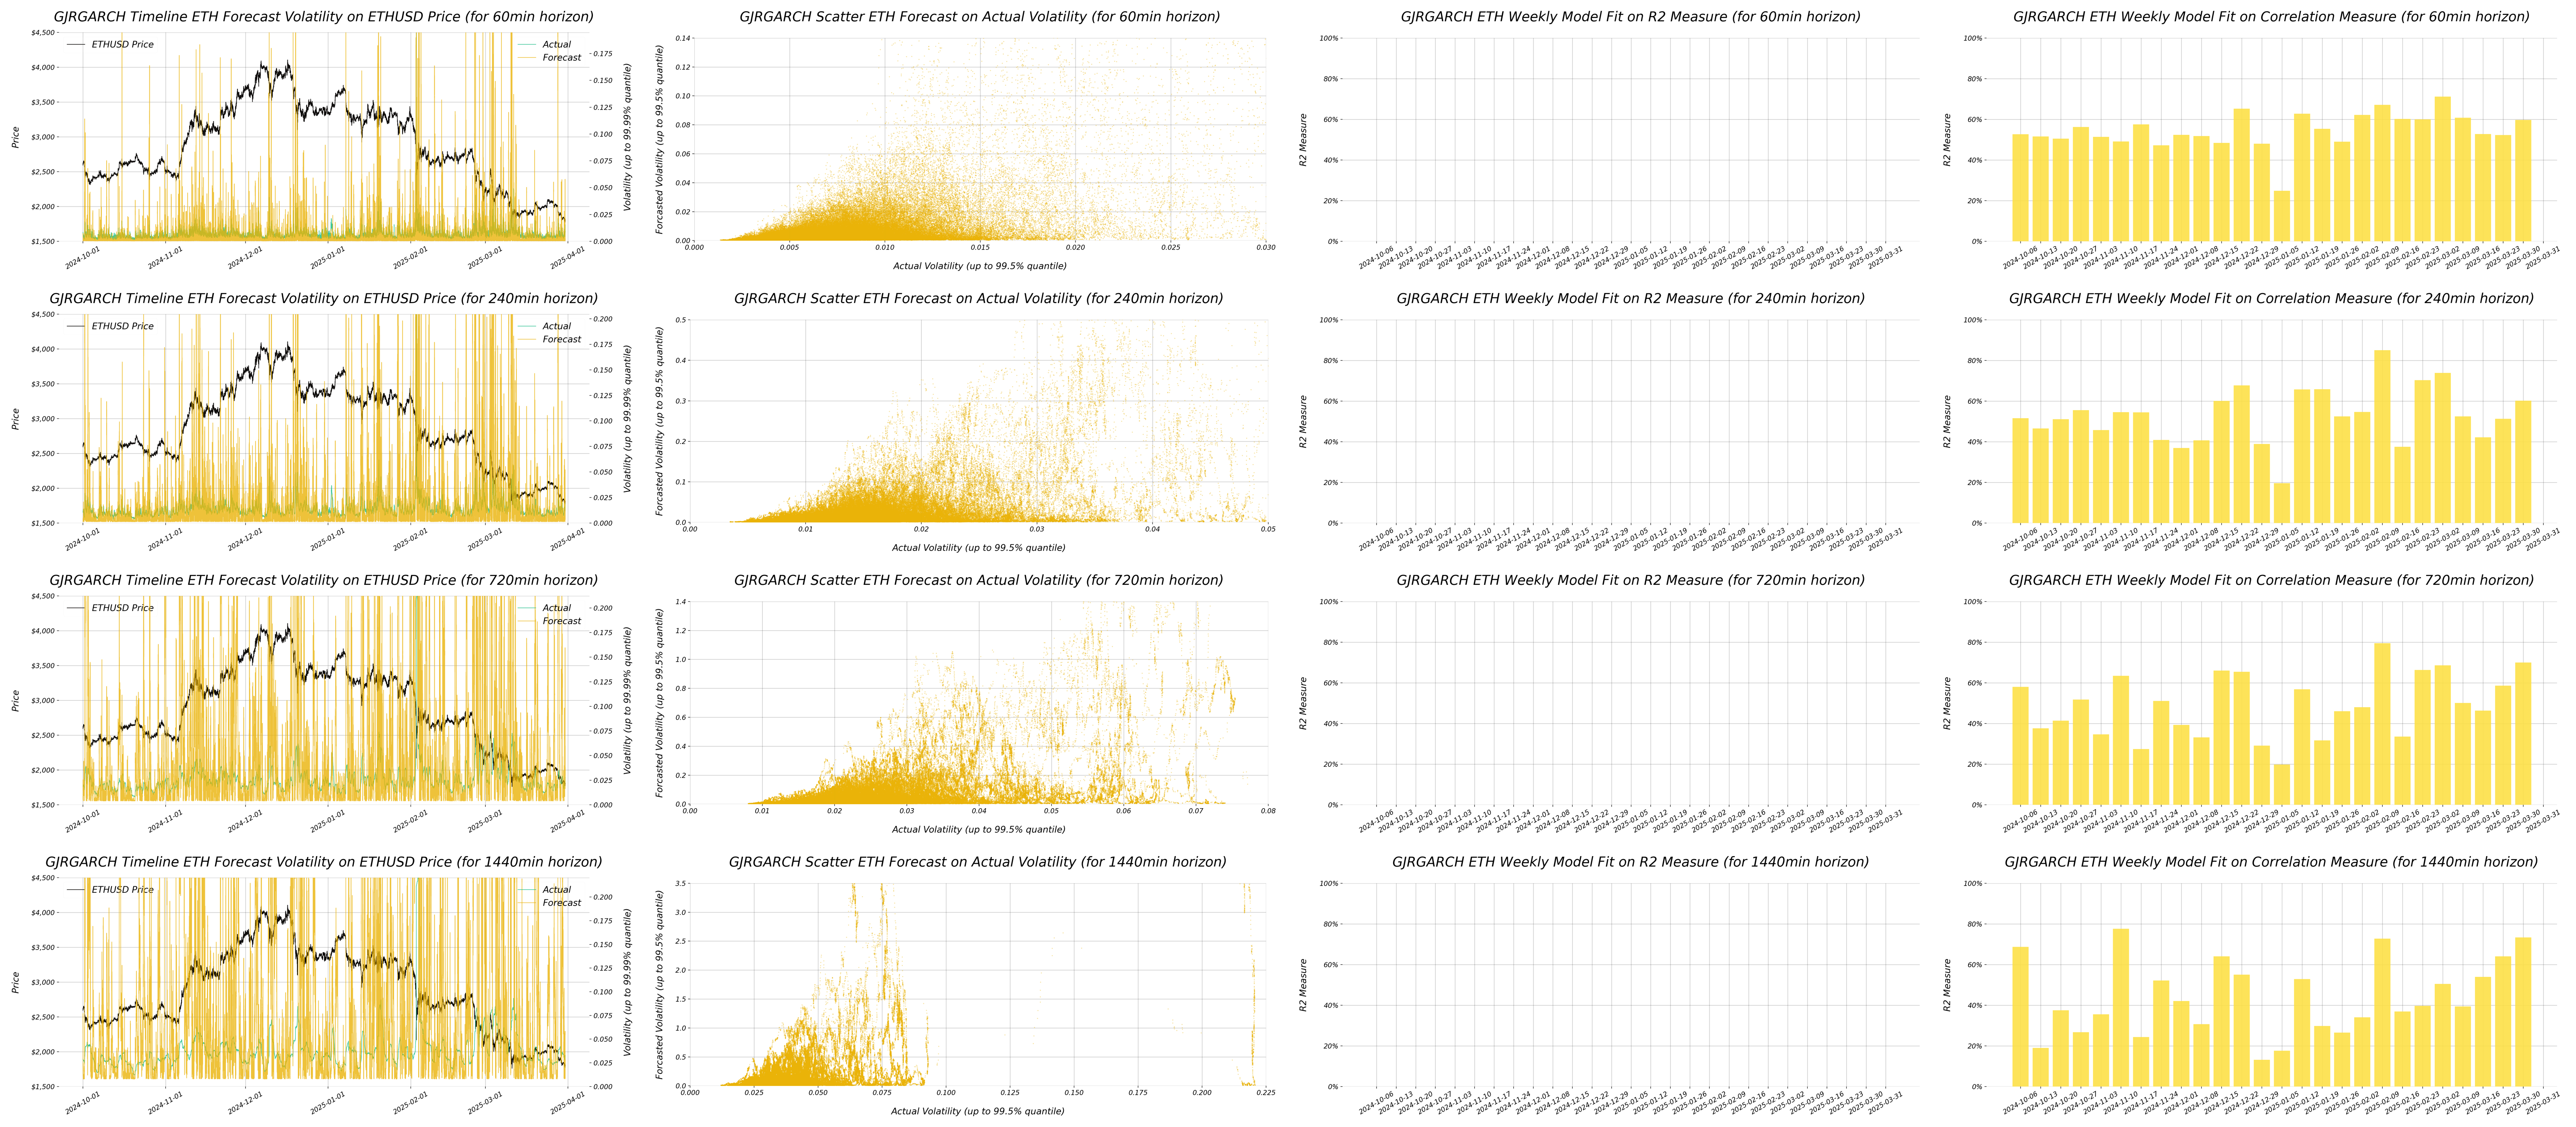
\includegraphics[width=.90\columnwidth]{img/_ETH GJRGARCH.png}
\captionof{figure}{Ethereum GJR-GARCH Forecasts Visualisation}
\label{fig:_ETH_GJRGARCH}

\end{document}